% Copyright (C) 2014-2016 by Thomas Auzinger <thomas@auzinger.name>

\documentclass[draft,final]{vutinfth} % Remove option 'final' to obtain debug information.
\setcounter{tocdepth}{2}

% Load packages to allow in- and output of non-ASCII characters.
\usepackage{lmodern}        % Use an extension of the original Computer Modern font to minimize the use of bitmapped letters.
\usepackage[T1]{fontenc}    % Determines font encoding of the output. Font packages have to be included before this line.
\usepackage[utf8]{inputenc} % Determines encoding of the input. All input files have to use UTF8 encoding.

% Extended LaTeX functionality is enables by including packages with \usepackage{...}.
\usepackage{amsmath}    % Extended typesetting of mathematical expression.
\usepackage{amssymb}    % Provides a multitude of mathematical symbols.
\usepackage{mathtools}  % Further extensions of mathematical typesetting.
\usepackage{microtype}  % Small-scale typographic enhancements.
\usepackage[inline]{enumitem} % User control over the layout of lists (itemize, enumerate, description).
\usepackage{multirow}   % Allows table elements to span several rows.
\usepackage{booktabs}   % Improves the typesettings of tables.
\usepackage{subcaption} % Allows the use of subfigures and enables their referencing.
\usepackage[ruled,linesnumbered,algochapter]{algorithm2e} % Enables the writing of pseudo code.
\usepackage[usenames,dvipsnames,table]{xcolor} % Allows the definition and use of colors. This package has to be included before tikz.
\usepackage{nag}       % Issues warnings when best practices in writing LaTeX documents are violated.
\usepackage{todonotes} % Provides tooltip-like todo notes.
\usepackage[pdftex,
            colorlinks=true]{hyperref} % Enables cross linking in the electronic document version. This package has to be included second to last.
\usepackage[acronym,toc]{glossaries} % Enables the generation of glossaries and lists fo acronyms. This package has to be included last.

%Source Code stuff
\usepackage[newfloat]{minted}
\usepackage{morewrites}
\usepackage[strings]{underscore} %BibTex doesn't like underscores in the URL
%\usepackage{float} % force figures to be placed in text

\newenvironment{code}{\captionsetup{type=listing}}{}
\SetupFloatingEnvironment{listing}{name=Source Code}

% Define convenience functions to use the author name and the thesis title in the PDF document properties.
\newcommand{\authorname}{Benedikt Wedenik} % The author name without titles.
\newcommand{\thesistitle}{A Big Data Analytics Framework for Evaluating Automated Elastic Scalability of the SMACK-Stack} % The title of the thesis. The English version should be used, if it exists.

% Set PDF document properties
\hypersetup{
    pdfpagelayout   = TwoPageRight,           % How the document is shown in PDF viewers (optional).
    linkbordercolor = {Melon},                % The color of the borders of boxes around crosslinks (optional).
    pdfauthor       = {\authorname},          % The author's name in the document properties (optional).
    pdftitle        = {\thesistitle},         % The document's title in the document properties (optional).
    pdfsubject      = {Master Thesis - SMACK Stack - Benedikt Wedenik},              % The document's subject in the document properties (optional).
    pdfkeywords     = {Big Data, Data Analytics, SMACK Stack, Scalability, Spark, Kafka, Akka, Cassandra, Mesos, DC/OS, Cloud Computing, Elasticity} % The document's keywords in the document properties (optional).
}

\setpnumwidth{2.5em}        % Avoid overfull hboxes in the table of contents (see memoir manual).
\setsecnumdepth{subsection} % Enumerate subsections.

\nonzeroparskip             % Create space between paragraphs (optional).
\setlength{\parindent}{0pt} % Remove paragraph identation (optional).

\makeindex      % Use an optional index.
\makeglossaries % Use an optional glossary.
%\glstocfalse   % Remove the glossaries from the table of contents.

% Set persons with 4 arguments:
%  {title before name}{name}{title after name}{gender}
%  where both titles are optional (i.e. can be given as empty brackets {}).
\setauthor{}{\authorname}{BSc}{male}
\setadvisor{Univ.Prof. Mag.rer.soc.oec. Dr.rer.soc.oec.}{Schahram Dustdar}{}{male}

% For bachelor and master theses:
\setfirstassistant{Projektass. Dipl.-Ing. Dr.techn.}{Stefan Nastic}{BSc}{male}

% Required data.
\setaddress{Muristrasse 87, 3006 Bern, Schweiz}
\setregnumber{1227151}
\setdate{24}{07}{2018} % Set date with 3 arguments: {day}{month}{year}.
\settitle{\thesistitle}{A Big Data Analytics Framework for Evaluating Automated Elastic Scalability of the SMACK-Stack} % Sets English and German version of the title (both can be English or German).
\setsubtitle{}{} % Sets English and German version of the subtitle (both can be English or German).

% Select the thesis type: bachelor / master / doctor / phd-school.
% Bachelor:
%\setthesis{bachelor}
%
% Master:
\setthesis{master}
\setmasterdegree{dipl.} % dipl. / rer.nat. / rer.soc.oec. / master
%
% Doctor:
%\setthesis{doctor}
%\setdoctordegree{rer.soc.oec.}% rer.nat. / techn. / rer.soc.oec.
%
% Doctor at the PhD School
%\setthesis{phd-school} % Deactivate non-English title pages (see below)

% For bachelor and master:
\setcurriculum{Software Engineering and Internet Computing}{Software Engineering and Internet Computing} % Sets the English and German name of the curriculum.

\begin{document}

\frontmatter % Switches to roman numbering.
% The structure of the thesis has to conform to
%  http://www.informatik.tuwien.ac.at/dekanat

\addtitlepage{naustrian} % German title page (not for dissertations at the PhD School).
\addtitlepage{english} % English title page.
\addstatementpage

\begin{acknowledgements*}
Working and writing a thesis in parallel consumes a lot of time and energy.
I want to thank my girlfriend Rita for supporting me during this time and being patient with me.\\
Further I want to thank Dr. Stefan Nastic for skillfully supporting me and giving me valuable feedback (even on the weekend).
Of course this thesis would have never been realized without the help of Prof. Schahram Dustdar.\\
At this point I want to emphasize the kind sponsoring of Zühlke Engineering AG in form of time, budget, real IoT data and expertise.\\
Last but not least I want to say that I'm grateful for my family and my friends for always believing in me.
\end{acknowledgements*}

\begin{kurzfassung}
In den letzten Jahren ist der Bedarf an schneller Verfügbarkeit von Informationen, sowie an kurzen Antwortzeiten gestiegen.
Die Anforderungen an ein heutiges Businesskonzept sind im Wandel: Stunden- oder gar tagelanges Warten auf die Ergebnisse einer Abfrage ist in vielen Branchen schlichtweg nicht mehr akzeptabel.
Die Antwort kommt sofort oder die Anfrage wird verworfen - genau hier setzt der Begriff "Fast Data" ein.
Mit dem SMACK Stack, bestehend aus Spark, Mesos, Akka, Cassandra und Kafka, wird eine robuste und vielseitige Datenverarbeitungsplattform bereitgestellt, auf der Fast Data Applikationen ausgeführt werden können.
In dieser Thesis wird ein Framework vorgestellt, mit dessen Hilfe Services und Ressourcen innerhalb des Stacks einfach skaliert werden können.
Die Hauptbeiträge können wie folgt zusammengefasst werden:
1) Entwicklung und Evaluation des genannten Frameworks, einschließlich der Monitoring-Metrik Extraktion \& Aggregation, sowie des Skalierungsservices selbst.
2) Implementierung zweier real-world Referenzapplikationen.
3) Bereitstellung von Infrastruktur-Management Tools mit deren Hilfe der Stack einfach in der Cloud deployt werden kann.
4) Bereitstellung von Deployment-Vorlagen in Form von Empfehlungen, wie der Stack initial am besten für die vorhandenen Ressourcen konfiguriert und gestartet wird.
Für die Evaluierung des Frameworks werden die zwei entwickelten real-world Applikationen herangezogen.
Die erste Applikation basiert auf der Verarbeitung von IoT Daten und ist stark I/O-lastig, während die zweite Applikation kleinere Datenmengen verarbeitet, dafür aber teurere Berechnungen durchführt, um Vorhersagen aufgrund der IoT Daten zu treffen.
Die Resultate zeigen, dass das Framework in der Lage ist zu erkennen, welcher Teil des Systems gerade unter hoher Last steht und diesen dann automatisch zu skalieren.
Bei der IoT Applikation konnte der Datendurchsatz um bis zu 73\% erhöht werden, während die Vorhersageapplikation in der Lage war bis zu 169\% mehr Nachrichten zu bearbeiten, wenn das Framework aktiviert wurde.
Obwohl die Resultate vielversprechend aussehen, gibt es noch Potenzial für weitere Verbesserungen, wie zum Beispiel der Einsatz von maschinellem Lernen um Schwellwerte intelligent anzupassen, oder eine breitere und erweiterte REST API.
\end{kurzfassung}

\begin{abstract}
In the last years the demand for information availability and shorter response times has been increasing.
Today's business requirements are changing: Waiting hours or even days for the result of a query is not acceptable anymore in many sectors.
The response needs to be immediate, or the query is discarded - This is where "Fast Data" begins.
With the SMACK Stack, consisting of Spark, Mesos, Akka, Cassandra and Kafka, a robust and versatile platform and toolset to successfully run Fast Data applications is provided.
In this thesis a framework to correctly scale services and distribute resources within the stack is introduced.
The main contributions of this thesis are:
1) Development and evaluation of the mentioned framework, including monitoring metrics extraction and aggregation, as well as the scaling service itself.
2) Implementation of two real-world reference applications.
3) Providing infrastructure management tools to easily deploy the stack in the cloud.
4) Deployment blueprints in form of recommendations on how to initially set up and configure available resources are provided.
To evaluate the framework, the real world applications are used for benchmarking.
One application is based on IoT data and is mainly I/O demanding, while the other one is computationally bound and provides predictions based on IoT data.
The results indicate, that the framework performs well in terms of identifying which component is under heavy stress and scaling it automatically.
This leads to an increase of throughput in the IoT application of up to 73\%, while the prediction application is able to handle up to 169\% more messages when using the supervising framework.
While the results look promising, there is still potential for future work, like using machine learning to better handle thresholds or an extended REST API.
\end{abstract}

% Select the language of the thesis, e.g., english or naustrian.
\selectlanguage{english}

% Add a table of contents (toc).
\tableofcontents % Starred version, i.e., \tableofcontents*, removes the self-entry.

% Switch to arabic numbering and start the enumeration of chapters in the table of content.
\mainmatter


%%%%%%%% CHAPTER %%%%%%%%%
\chapter{Introduction}
\label{ch:introduction}

\section{Motivation \& Problem Statement}
\label{sec:motivation}
In the last years the demand of information availability and shorter response times is increasing.
Existing problems, such as the large amount of data to process and analyze in a big data application, are not the only challenges to solve.
There are many sensors, mobile devices and other IoT devices out in the field, constantly sending data in form of streams to the processing servers.\\
Today's business requirements are changing: Waiting hours or even days for the result of a query is not acceptable anymore in many sectors.
The response needs to be immediate, or the query is discarded \cite{estrada2016big}.
Quick responses, ideally near real-time, are crucial success factors.
Many data warehouses are facing the problem that the stored data is slowly becoming obsolete.
This is why "Fast Data", as an approach to solve those problems, increases its popularity, as being "big data, but fast" \cite{mishne2013fast}. \\


The SMACK-Stack consists of five technologies combined to a lightning fast data pipeline for today's needs of big data applications.\\
\begin{itemize}
    \item Apache \textbf{S}park is the engine of the pipeline, providing batch-, as well as stream-processing power for large-scale data processing.
    \item \textbf{M}esos is a datacenter operating system with the aim to reduce complexity and ease the deployment and maintenance of large-scale distributed applications.\\
    \item Apache \textbf{A}kka can be seen as the model, providing the possibility to build powerful reactive distributed message-driven applications.\\
    \item Apache \textbf{C}assandra is a highly distributed database which is a hybrid between a column-oriented and a key-value DBMS, which is implemented avoiding a single point of failure.\\
    \item Apache \textbf{K}afka serves as publish-subscribe message broker, which is usually the ingestion point of the pipeline.\\
\end{itemize}


\section{Motivating Scenarios}
To evaluate the framework developed in the course of this thesis, an extensive evaluation is performed.
The setup contains two real world applications, which serve as a basis for benchmarking and exploring the optimal resource distribution when scaling up and down.
One application is I/O-bound, which means there is not a lot of logic inside the data pipeline, but many requests have to be processed, which is done with real world IoT data.
The other one is a computational bound application, which does not have to deal with many requests in parallel but requires a lot of computation power inside the pipeline.

\subsection{Real World IoT Data Storage Application}
\label{sec:iot_application}
During the HackZurich 2016 \cite{hackzurich_website}, Europe's largest hacking contest, Zuehlke Engineering AG \cite{zuehlke} developed a simple real world IoT application to be used with SMACK \cite{hackzurich}.\\
The application can be categorized as sensor data ingestion and analysis software.
It is designed to run in a cluster and handle vast amounts of incoming data.\\
As this is the product of a hackathon, the initial state was only a very basic implementation and had to be extended to fit the needs of this thesis.\\

In abstract terms, the application serves as endpoint for ingesting and storing relevant IoT data.
The devices connect and send their data via HTTP to a REST endpoint.
After this, the data pipeline processes and normalizes the input to finally store the data into the Cassandra database for later analysis or statistical evaluation.\\

Figure~\ref{fig:hackzurich} gives a rough overview of how the single components of SMACK are interacting with each other in this application.
In Figure~\ref{fig:iot} a more detailed view gives insight of how the application is designed.\\
All the IoT devices are sending their data in JSON the REST webservice named \textit{sensor-ingestion}, implemented using Akka actors.
The reason to use Akka is to be able to provide a reactive application without a lot of manual programming effort.
While the JSON input is not parsed in Akka it is simply transferred to a Kafka topic - in this case to the topic \textit{sensor-reading} - to be processed later on in Spark.\\
This means that Kafka servers as a buffer here to allow the ingestion to be decoupled from the processing.
In the Spark job, which is called \textit{KafkaToCassandra}, the JSON is parsed and validated and then send to Cassandra to be stored in the \textit{sensordata} keyspace for later analysis.\\

A handy tool to interact with Cassandra and to perform real-time data analysis, is Apache Zeppelin, which provides interactive scratch books and can be used with most modern big data technologies.
There are some example scratch books in the repository, which can be used in the context of the sensor data application.\\

All commits can be found in the repository \cite{hackzurich}, but the main contribution to this application can be summarized in the following points:
\begin{itemize}
    \item Fixing compile errors and updating dependencies
    \item Updating docker image creation
    \item Collecting and computing statistics / metrics for the application
    \item Adding a feature to export metrics of the sensor ingestion via JMX
    \item Extension of the existing load generator.\\
          The JSON files are now compacted to be able to achieve higher throughputs and use less CPU on the client side.
          Further the input handling of those files had to be adjusted.
\end{itemize}

The application can be categorized as real world application, because real IoT sensor data has been recorded and can be used again for later stress testing.
Further the scenario is not artificial - in the context of the HackZurich, a company producing and maintaining elevators used this application to gather information about their products to use it for predictive maintenance.\\
As it can be seen from the context of the application, consistency in terms of not losing a single sensor data is not required.
It is required though, that the system stays reactive and responsive even under heavy load and is capable of handling the data in a fault-tolerant way.
For example if one node goes offline, the whole data pipeline must not be disturbed, as it would mean that data loss occurs.
Further the persistence is a highly desired property in this scenario.
The data must be stored securely, so that the data scientists can later on perform their analysis for the predictive maintenance, even when the stack goes offline.

\begin{figure}[!htbp]
  \centering
  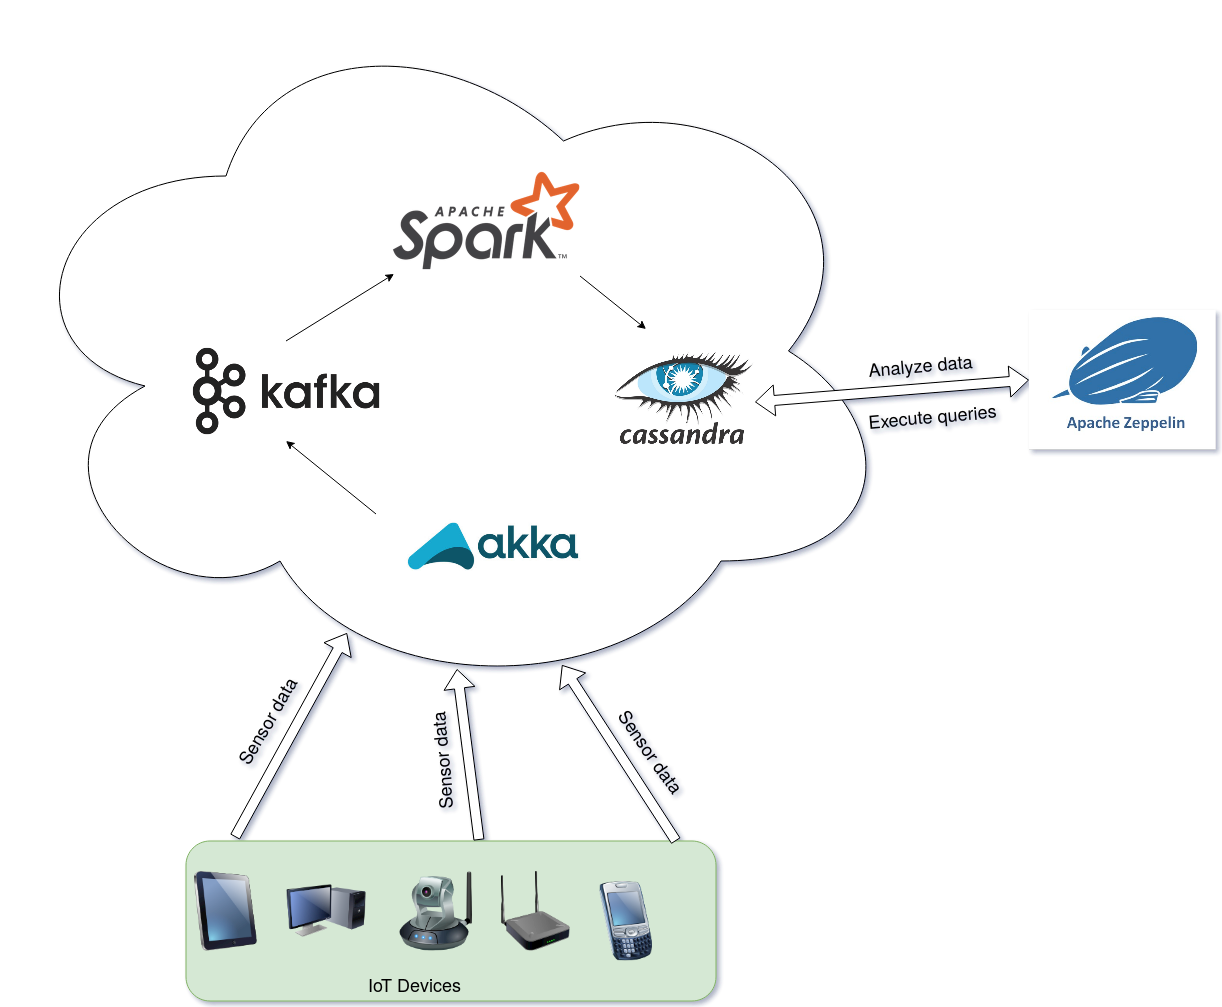
\includegraphics[keepaspectratio=true,scale=0.38]{img/hackzurich}
    \caption{Abstract View of Zuehlke HackZurich IoT Application}
  \label{fig:hackzurich}
\end{figure}

\begin{figure}[!htbp]
  \centering
  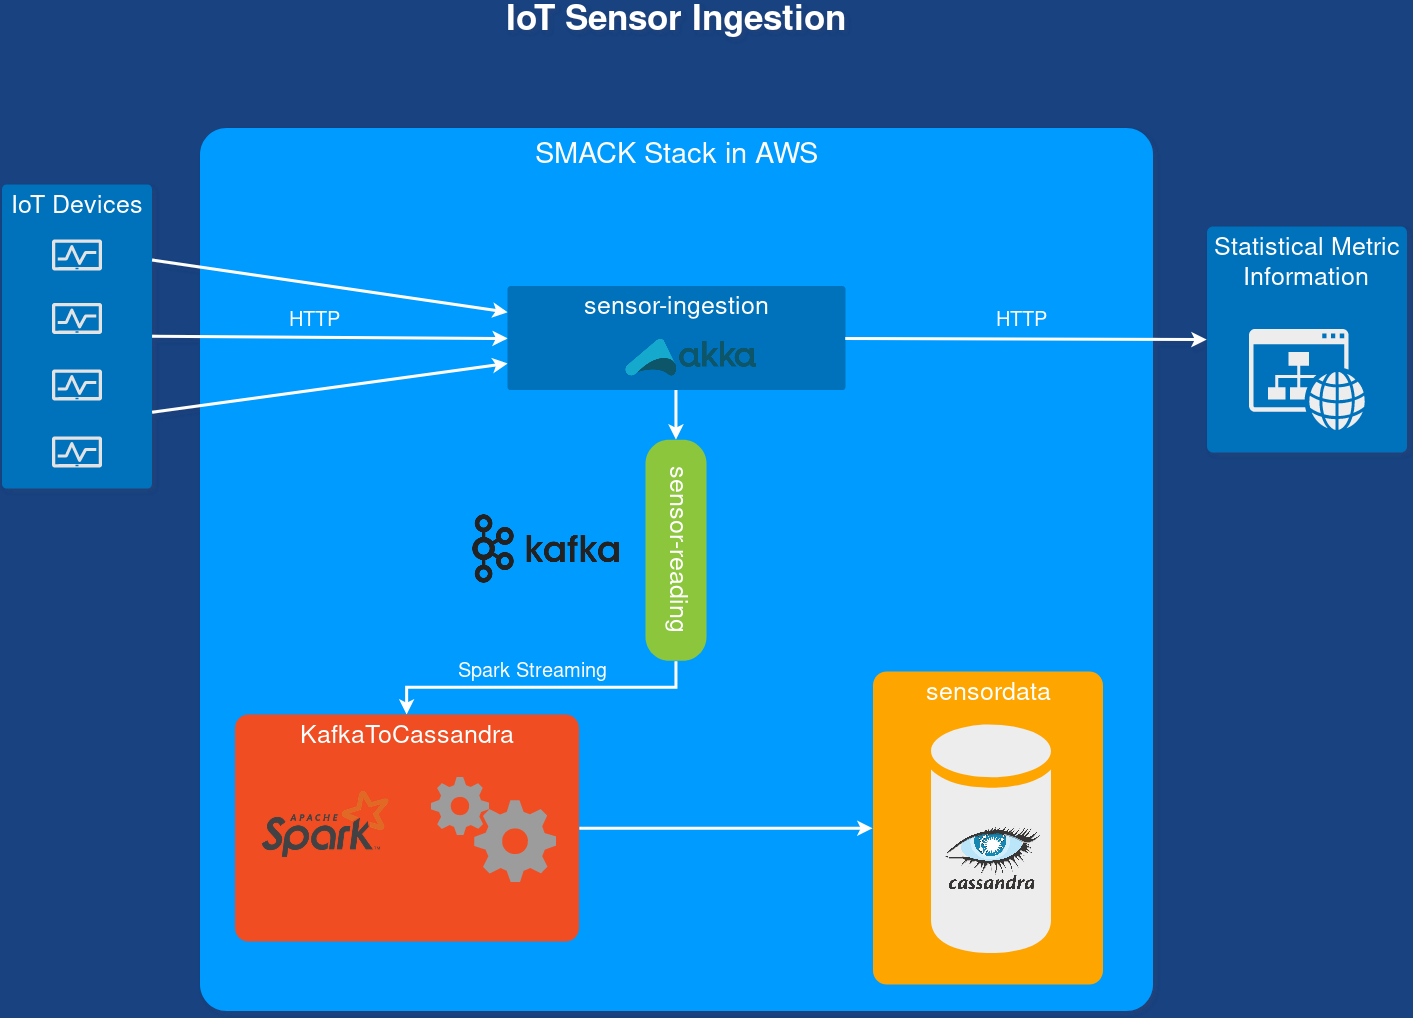
\includegraphics[keepaspectratio=true,scale=0.35]{img/IoT}
    \caption{Detailed View of the Zuehlke HackZurich IoT Application}
  \label{fig:iot}
\end{figure}


\subsection{Real World Acceleration Prediction Application}
\label{sec:computation_application}
In the course of this thesis, a new application was developed which is mainly computational bound and handles less input data than the IoT application.
The IoT application is used as a base, including the real life data, but as mentioned, just a fraction of the volume is ingested.\\
Information about how the data looks like in detail can be found in section \ref{sec:sensor-data}.\\

To provide a realistic use case, this application learns from the past and predicts the movements of the elevators in the future.
This could be especially helpful when talking about predictive maintenance or even more when optimizing the idle time of the elevators.
Imagine the waiting times at an elevator can be reduced because it automatically starts to move up or down based on the prediction.
In most cases, the elevator would be in movement even before the real request by a user would occur.\\
The application is written in Scala and Spark using an ARIMA model of the spark-timeseries library.
Information about the history is gathered from the Cassandra database, which is filled with data by using the light-weighted version of the IoT application.\\

Figure~\ref{fig:prediction} illustrates the architecture of the whole application.\\
As one can see, the ingestion part is the same as in the IoT application as mentioned above.
The data is ingested by the \textit{sensor-ingestion} application based on Akka, which writes in the \textit{sensor-reading} Kafka topic.
From there the \textit{KafkaToAccelerometer} Spark job constantly receives data via Spark Streaming and writes the processed data into the \textit{sensordata} keyspace of Cassandra, as well as publishing the latest processed accelerometer data into the \textit{sensor-reading-accelerometer} Kafka topic.\\
The \textit{Prediction Data Analytics} Spark job constantly polls from Cassandra and calculates the predictions based on the available data.
The results are written into the \textit{data-analytics} topic.
In the \textit{akka-data-analytics} application the results of the slower but more precise prediction from Spark are polled.
Additionally the application performs a basic prediction with the help of linear regression, based on the available data from the \textit{sensor-reading-accelerometer} topic.\\
This design is related to the Lambda architecture, which uses a speed and a batch layer, to be able to constantly provide results to the end user.
In the application, both predictions are combined if available.
If there is just data from the "speed layer" or just the "batch layer" this data is published via HTTP to the end user.
In case both layers provide data for the same timestamp, the values are combined with the help of weights, ${speed} * 0.3 + {batch} * 0.7$.\\

In order to generate a satisfying amount of datasets the application only considers \textit{Accelerometer} data, as this data occurrs most frequently in the real-life dataset.
Additionally the information about the acceleration is enough to provide predictive values of when the elevator should start to move up or down.

\begin{figure}[!htbp]
  \centering
  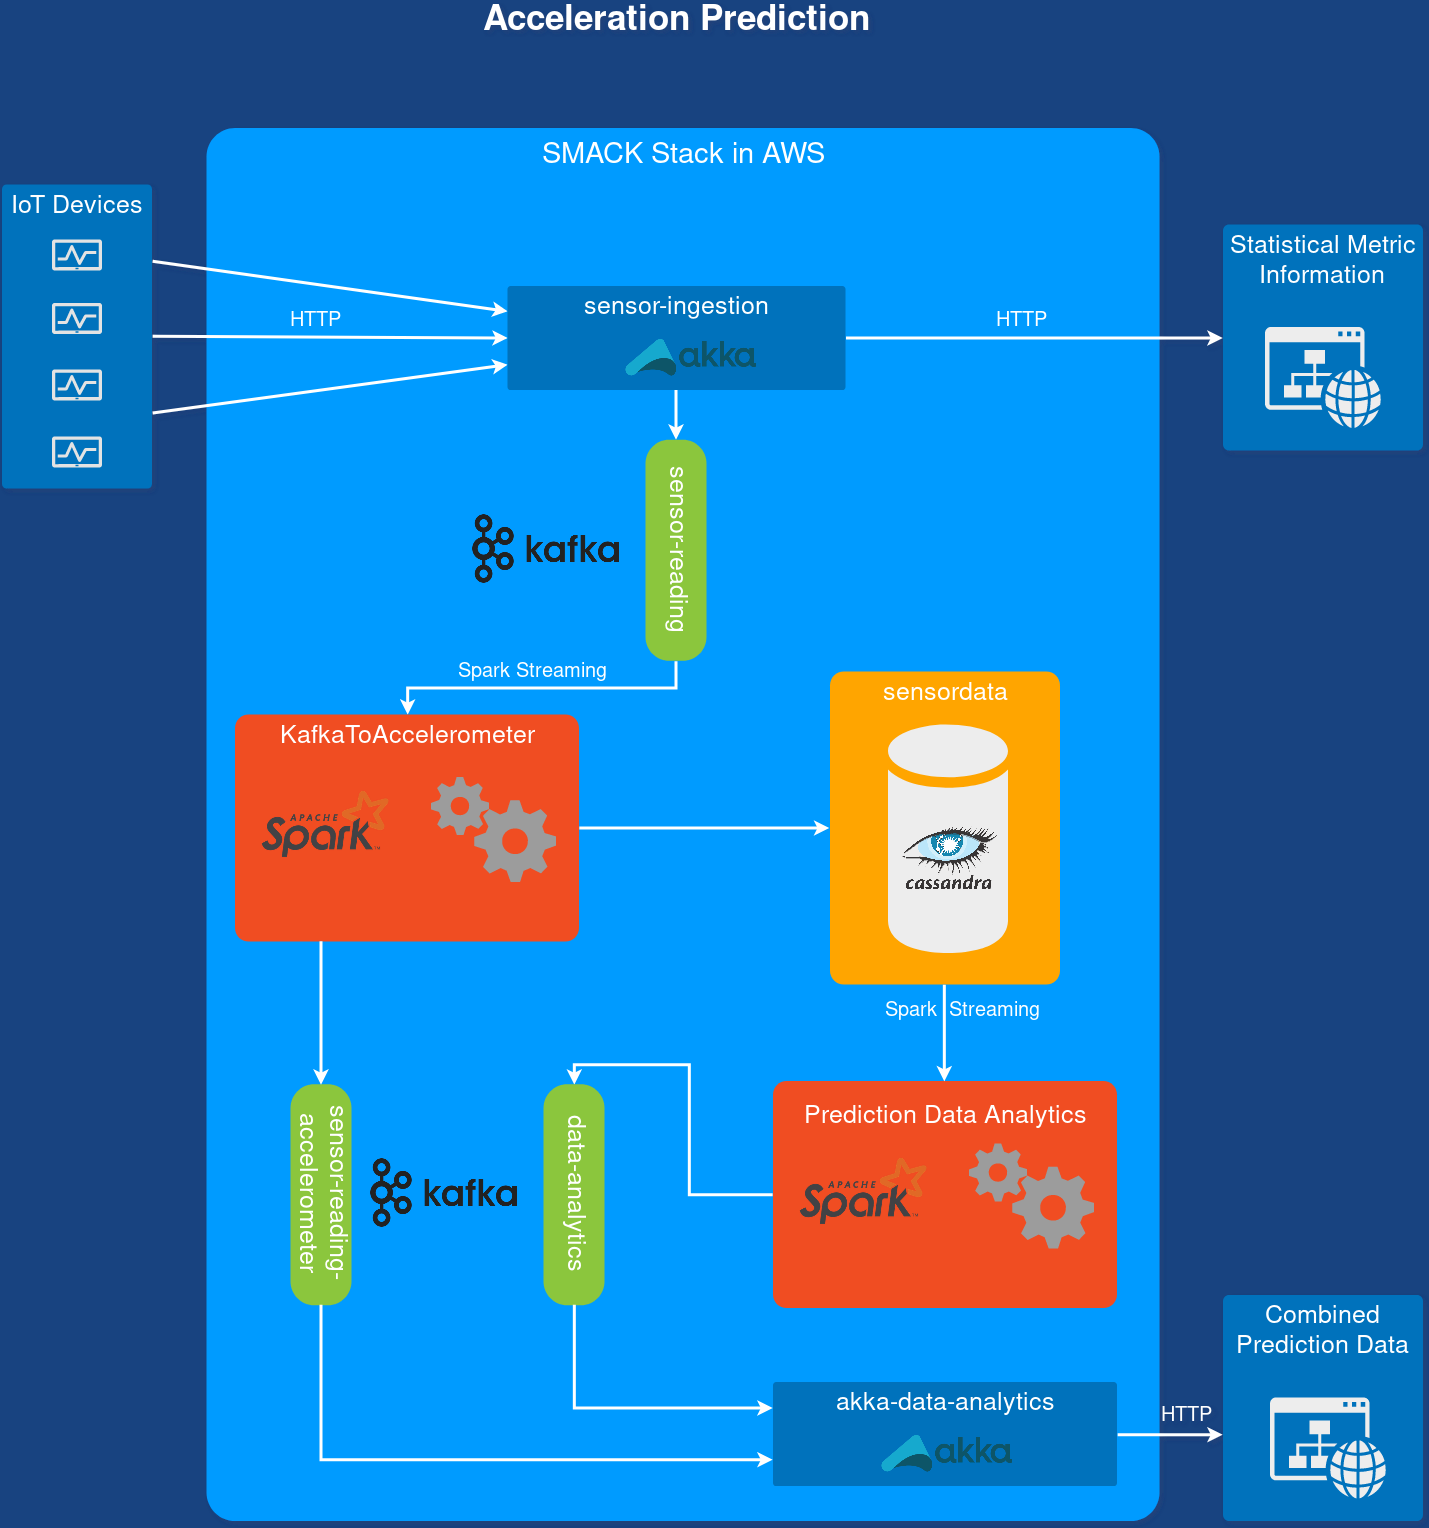
\includegraphics[keepaspectratio=true,scale=0.33]{img/prediction}
    \caption{Detailed View of the Acceleration Prediction Application}
  \label{fig:prediction}
\end{figure}


To measure the quality of the predictions, a \textit{Kolmogorov Smirnov Test} is done \cite{wilcox2005kolmogorov}.
The setup of the test looks like follows:\\
\begin{enumerate}
    \item Select only those values for which a prediction and the real value is given for the same timestamp (and obviously the same elevator/device).
    \item Accumulate the values of the dataset, where $x$ are the timestamps and $y$ are corresponding values.\\
          $c_1 = y_1$\\
          $c_2 = c_1 + y_2$\\
          $c_n = c_{n-1} + y_n$\\
          ...
    \item Create a new dataset which consists of the same x-values and for each y-value calculate $y_{diff} = abs(y_{real} - y_{prediction})$.
    \item Now we can calculate the minimum, maximum and average of the differences and add this curve to the plot.
\end{enumerate}

For an easy and illustrative comparison of the real versus the predicted data, the Kolmogorov Smirnov Test is plotted in Figure~\ref{fig:prediction_vs_real}, where the following statistical values apply with respect to the calculated difference-curve:\\
${Min}: 0.04$\\
${Max}: 8.56$\\
${Avg}: 5.05$\\

The K.S. Test indicates that the prediction is promising.
One can observe that the curves develop very similar but are a bit biased.
The compensation or removal of this bias could be a possible further improvement for future work.
Still the K.S.-Test confirms, that the prediction is not "random output" and has a measurable correlation to the real values.

\begin{figure}[!htbp]
  \centering
  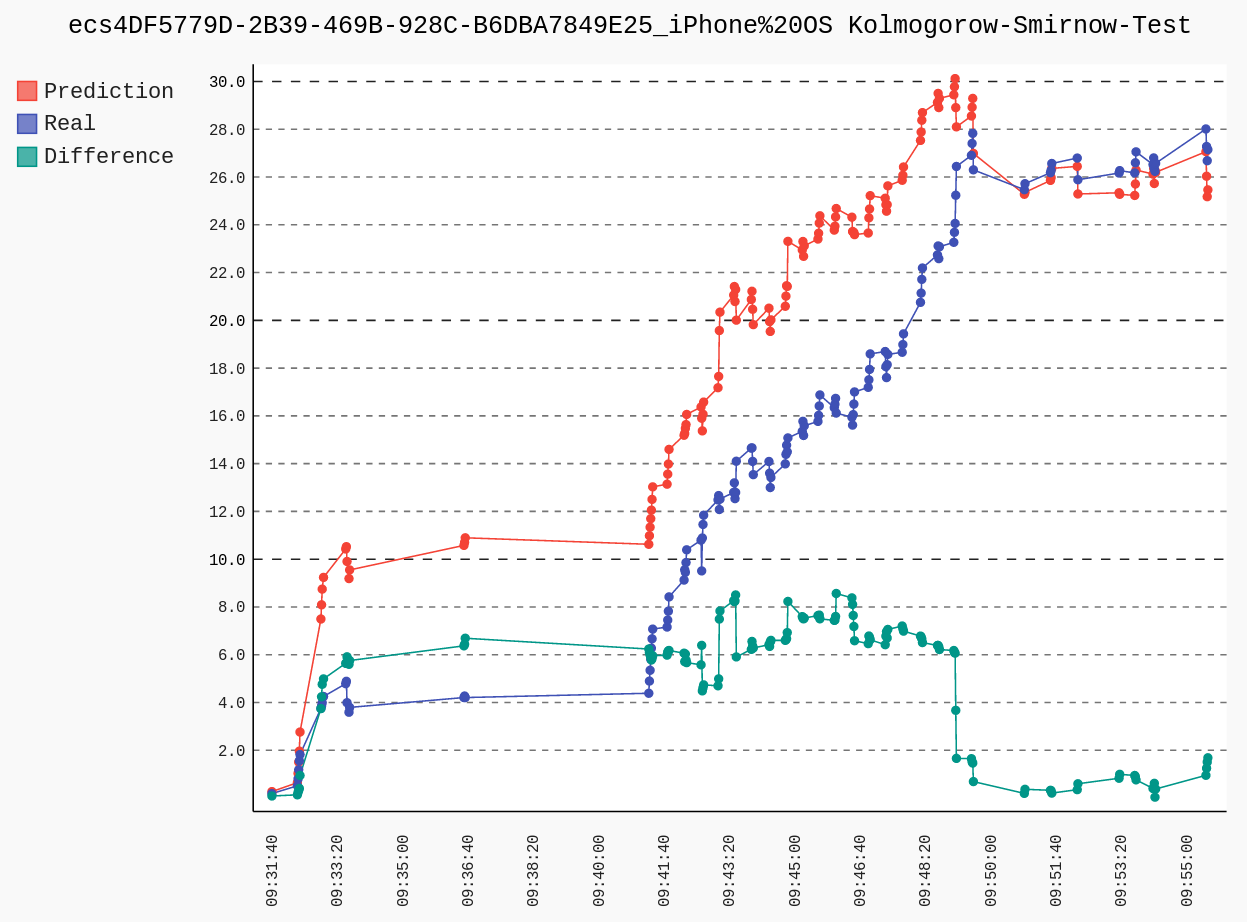
\includegraphics[keepaspectratio=true,scale=0.36]{img/prediction_vs_real}
    \caption{Kolmogorov Smirnov Test - Prediction versus Real}
  \label{fig:prediction_vs_real}
\end{figure}


\section{Research Challenges}
In terms of operating and managing a cluster there are a various challenges, developers and system administrators are faced with.\\
\begin{itemize}
    \item Deploying large scale applications\\
          When facing the challenge of deploying productive applications in a large scale cluster, several factors need to be considered.
          Many applications consist of multiple instances of different technologies, or are hosted in various Docker containers.
          The deployment needs to be performed in a defined sequence to fulfill subsequent dependencies.
          In addition, depending on the used cluster manager, a lot of manual steps are required until the application is ready and online.
    \item Initial setup\\
          The decision of how to configure the instances of an application is a non-trivial task, as there are almost infinite combination possibilities and the impact can be drastic.
          Finding the right distribution of resources within a cluster across the hosted applications can be a challenging task.
          This is especially crucial when the deployed application deals with large amounts of data and clients, while still staying responsive and fault-tolerant.
    \item Monitoring\\
          There are many tools available to monitor clusters and big data applications, although a deeper understanding of the used frameworks is required.
          Considering just RAM, CPU and disk usage is in most cases insufficient.
          For example, a high usage of RAM in a Spark Job would not necessarily mean that it is under heavy load, but that Spark uses - per design - a lot of memory to leverage it's computation power, compared to disk intensive frameworks like Hadoop.
          This introduces a new layer of complexity, as each framework has its own characteristics and metrics to observe when monitoring a cluster.
          Understanding what's going on in a cluster and reacting accordingly is crucial for the success of any large scale application.
    \item Scaling when needed\\
          Recognizing when to scale which component of an application is a 24/7 task.
          In the ideal case, the system automatically scales up and down as required.
          There are many existing approaches, but the quality of the automated scaling still relies heavily on the quality and significance of the monitored metrics.
          Without the right metrics, the scaling cannot be reliable and thus requires most of the time manual decisions.
\end{itemize}

All the components of the SMACK stack proved that they are very scalable used in isolation.
Now the question is, where is the bottleneck when using them as combined data pipeline?
Another important question is how to distribute the resources in an optimal way.
For example if there is an application running in the cloud, how should the CPU, RAM, disk space etc. be assigned to the different technologies to achieve the best performance for the lowest price.
Of course this question can only be answer with respect to the requirements of the application and the kind of data to process, i.e. the input data pattern.
This is where a framework can be developed to automatically analyze and regulate resource allocation for the SMACK stack.\\


\section{Background}
This section givs an overview of the single components of the SMACK stack, namely Spark, Mesos, Akka, Cassandra and Kafka.
A basic knowledge of the used technologies is crucial for the reader to be able to understand the complex interdependencies which are omnipresent when using a big data stack with multiple technologies.

\subsection{Akka}
"Akka is a toolkit for building highly concurrent, distributed, and resilient message-driven applications for Java and Scala" \cite{akka_web}.\\
The mathematical model behind Akka is the \textit{Actor Model}, which was developed and presented in the first place by C. Hewitt, P. Bishop and R. Steiger in 1973 \cite{hewitt1973session}.
During the time the paper was written, hardware was very expensive, which is not the case anymore today.
As a consequence, implementing large scale systems processing millions of requests per second is now possible in a cheap fashion.\\

One can imagine actors as objects which are receiving and sending messages between each other.
Because in theory the order of the messages is not relevant, the behavior of statelessly handling messages is encouraged.
The Akka implementation provides a so called \textit{mailbox}, in which messages are stored to be processed later in case an actor receives multiple messages at once.
These mailboxes usually have a limit after which newly received messages are simply dropped.
An actor can internally handle and process a message, but can also forward it to another actor, or even create a new actor to help achieving the required task.\\

According to the official Akka website, akka.io, the provided framework is the defacto-standard implementation of the actor model and comes with some interesting key features in aspect of big data \cite{akka_web}.
The framework is designed to be resilient by design, which allows developers to implement self-healing and responsive applications with ease.
Further the website claims to prodive capacity handling of 50 million messages per second on a single machine, while one GB of available heap can host up to 2.5 million actors.
This in combination with the asynchronous nature of the model provides a powerful platform to build responsive and highly scalable big data applications.


\subsection{Apache Spark}
"Apache Spark is a fast and general engine for large-scale data processing" \cite{apache_spark}. \\
Build for big data processing, this open-source framework offers the possibility outperform existing Hadoop solutions with ease.
"It has emerged as the next generation big data processing engine, overtaking Hadoop MapReduce which helped ignite the big data revolution.
Spark maintains MapReduce's linear scalability and fault tolerance, but extends it in a few important ways: it is much faster (100 times faster for certain applications)" \cite{shanahan2015large}.
The main reason for the immense speed is the build in direct acyclic graph execution engine, which supports in-memory computing, as well as acyclic data flows.\\

One big advantage of Spark is it's rich set of APIs, like Scala, Java, Python, R etc.
There are over 80 high-level operators, which allows developers to easily build robust and highly parallel applications.
For trying out new concepts or algorithms, there is an interactive mode, the so called Spark-shell. \\

In addition to the Spark core, there it consists of four main components:

\begin{itemize}
\item Spark SQL\\
This module allows the developer to work with structured data.
It provides seamless integration of Spark programs with SQL queries.
Another very powerful feature of Spark SQL is that one can uniformly access data, which means that there is just one common way to access all kind of supported data sources.
An example could be loading a JSON file is from Amazon S3 and used later as a table in an SQL query.\\
Further it is also possible to use JDBCS or ODBC drivers to connect ones business application to Spark.

\item Spark Streaming\\
The goal of this component is to provide both, fault-tolerance and scalability for streaming applications.
Through build-in high-level operators, it is possible to write streaming jobs in the same way one would implement a batch job.
A very powerful feature is the automatic recovery strategies - Spark recovers the state of the application as well as the lost worker node without requiring any additional code.
This is enables the developers to focus on what they want to implement on don't have to deal with complex fault tolerance for each component.\\
Again, it is possible to use the same code for batch, stream or ad-hoc queries, which leads to the possibility of building interactive applications without a lot of effort.

\item MLib\\
The integrated machine learning library provides many high quality algorithms, implemented to be efficient out of the box.
It's up to 100 times faster than traditional MapReduce approaches, such as Hadoop.
The dramatic runtime comparison difference can be seen in Figure~\ref{fig:spark_vs_hadoop}.


\begin{figure}[!htbp]
  \centering
  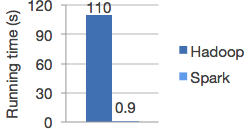
\includegraphics[keepaspectratio=true,scale=0.7]{img/spark_vs_hadoop}
    \caption{Spark vs. Hadoop - "Logistic regression in Hadoop and Spark" \cite{apache_spark}}
  \label{fig:spark_vs_hadoop}
\end{figure}

\item GraphX\\
    This API is designed to allow graph-parallel computation in combination with collections a seamless way.
    Thanks to the community the library of graph algorithms is growing and openly available for everyone.
    In terms of speed, the GraphX implementations can be compared with other state of the art graph libraries, which is illustrated in Figure~\ref{fig:spark_graphx}.

\begin{figure}[!htbp]
  \centering
  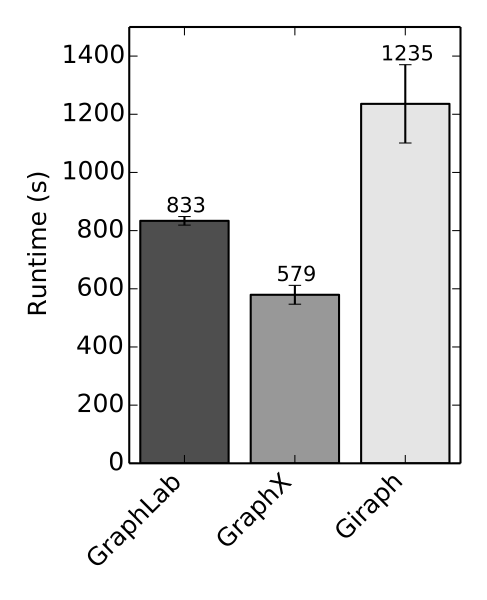
\includegraphics[keepaspectratio=true,scale=0.5]{img/spark_graphx}
    \caption{"End-to-end PageRank performance (20 iterations, 3.7B edges)" \cite{apache_spark}}
  \label{fig:spark_graphx}
\end{figure}

\end{itemize}

\textbf{Spark Architecture}\\
Figure~\ref{fig:spark_cluster_overview} illustrates the general architecture of any Spark program, regardless whether running in standalone or cluster mode.
The driver program is responsible for creating and executing operations on the so called Resilient Distributed Datasets (RDD), which are a main feature of Spark.
RDDs are abstractions of parallelized collections and have some powerful characteristic, especially when dealing with Big Data.
Those data structures are immutable, resilient, use lazy evaluation, are process aware and live in memory.\\
In addition, the driver is also responsible for creating and maintaining the Spark context, which is necessary for the connection between the nodes and the cluster.
Further configuration settings can be passed to the context during initialization, which affect the whole Spark program.
In our case, the cluster manager will be Mesos, which is responsible for launching and distributing the executors.\\
As the figure shows, each executor can run multiple tasks and usually in cluster mode, each executor is placed on a different worker node to provide even more fault-tolerance in case a node dies unexpectedly, but this behaviour can of course be overwritten manually.
If the driver node dies, the whole Spark program will be shutdown.
For this case a dedicated recovery strategy would have to be set up and implemented.

\begin{figure}[!htbp]
  \centering
  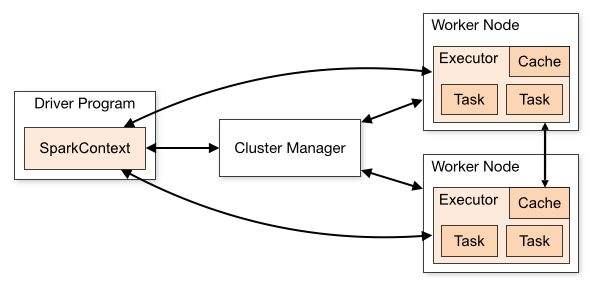
\includegraphics[keepaspectratio=true,scale=0.6]{img/spark_cluster_overview}
    \caption{Spark cluster with two executor nodes \cite{apache_spark}}
  \label{fig:spark_cluster_overview}
\end{figure}


\subsection{Apache Cassandra}
"Apache Cassandra is a free and open-source distributed NoSQL database management system designed to handle large amounts of data across many commodity servers, providing high availability with no single point of failure" \cite{cassandra_wikipedia}.\\
Many big companies, like eBay, Netflix, GitHub, etc. rely on the power of Cassandra to manage and store their data.
The masterless design offers flexibility as the cluster can be scaled up and down without any down time.
In Cassandra, the key-value and column oriented approach is combined to achieve extra performance when reading and writing data.\\
Research has been done concerning the speed of Cassandra: "In terms of scalability, there is a clear winner throughout our experiments.
Cassandra achieves the highest throughput for the maximum number of nodes in all experiments with a linear increasing throughput from 1 to 12 node" \cite{rabl2012solving}.\\
Due to the automatic replication of data onto multiple nodes, fault-tolerance is ensured.
In addition there is also support for replication across data center.\\
Cassandra comes with a custom Cassandra Query Language (CQL), which was designed to be close to what most developers know very well - regular SQL.

\begin{figure}[!htbp]
  \centering
  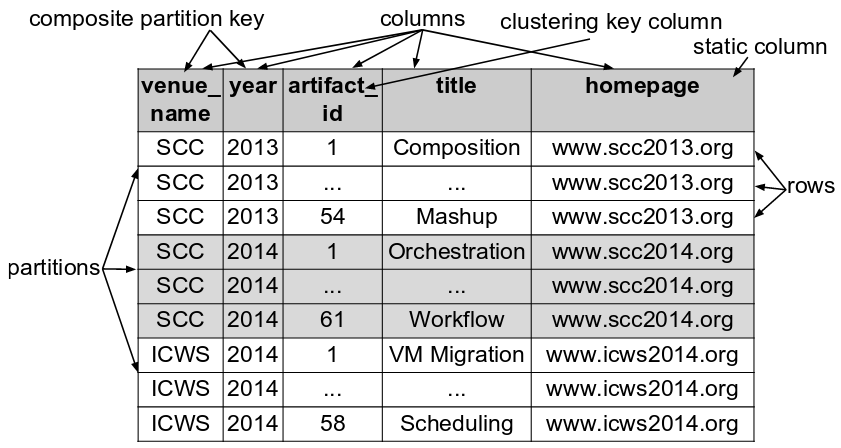
\includegraphics[keepaspectratio=true,scale=0.4]{img/cassandra_table}
    \caption{Cassandra Table \cite{chebotko2015big}}
  \label{fig:cassandra_table}
\end{figure}

As the data model is a mix between columns and key-value pairs, one has to keep in mind basic design decisions based on this structure.
An illustrative table is displayed in Figure~\ref{fig:cassandra_table}, showing the key concepts of how data is structured in Cassandra.
To be able to distribute data across nodes, it is required to define a \textit{Partition Key}, which is in this case a composition between \verb|venue_name| and \verb|year|.
This explains why there are exactly three partitions in the given table.\\
The \textit{Clustering Key}, in our case \verb|artifact_id|, is responsible to tell Cassandra how to sort data within the partition, which can be seen in the table.
Using the \textit{static} keyword, tells Cassandra to associate the respective column directly to the partition key and not - as by default - to the clustering key.
This behaviour is desired, when one wants to update this column for all entries in the same partition.


\subsection{Kafka}
"Kafka is used for building real-time data pipelines and streaming apps.
It is horizontally scalable, fault-tolerant, wicked fast, and runs in production in thousands of companies" \cite{apache_kafka}.\\
The main characteristics of this framework can be summarized as follows \cite{estrada2016big}:
\begin{itemize}
    \item Distributed. Scaling up horizontally without any downtime is important for a Big Data framework.
        Kafka is designed to run in a cluster with one or multiple nodes.
    \item Multiclient. To make the platform attractive for many developers, many programming languages are supported, like Java, Python, PHP, .NET, etc.
    \item Persistent. The fault-tolerant design prevents data loss, even when a node dies.
    \item Real time. Kafka is designed to provide data structures with efficiency of $\mathcal{O}(1)$, regardless of the data size.
        Using so called \textit{complex event processing}, produced messages are transmitted immediately to the customers.
    \item High throughput. The performant design allows this framework to handle hundrets of reads and writes per second, even with many clients in parallel.
\end{itemize}

Kafka provides four core APIs, namely Producer, Consumer, Streams and Connector.
A producer publishes streams containing records to so called topics, while the consumer is subscribed to one or more topics and reads the stream.
With the Streams API the possibility of directly transforming an input stream in an output stream is given.
To be able to interact with other systems, like for example a Cassandra database, the Connector API enables the developer to hook in and run reusable producers and consumers interacting with Kafka.\\
To be able to run in a cluster, Kafka relies on \textit{ZooKeeper}, which is a "distributed, open-source coordination service for distributed applications" \cite{apache_zookeeper}.\\
Every cluster setup consists of the following five components:
\begin{itemize}
    \item Topic. The central element in which streams of records are published by a producer and read by the consumer.
        Partitioning is the key to provide fault-tolerance and each partition contains a ordered sequence of immutable messages.
    \item Broker. The server process of Kafka is called broker and handles requests of producers and consumers, while the topics reside inside the broker.
    \item Producer. As mentioned above, the produces sends messages to the broker who stores them in chronological order into the respective topic.
    \item Consumer. Requests data from topics and processes the incoming data stream.
    \item ZooKeeper. Is the coordinator between the consumers and Kafka brokers.
\end{itemize}

Figure~\ref{fig:kafka_multinode_multibroker} shows how the architecture with multiple brokers running on multiple nodes could look like.

\begin{figure}[!htbp]
  \centering
  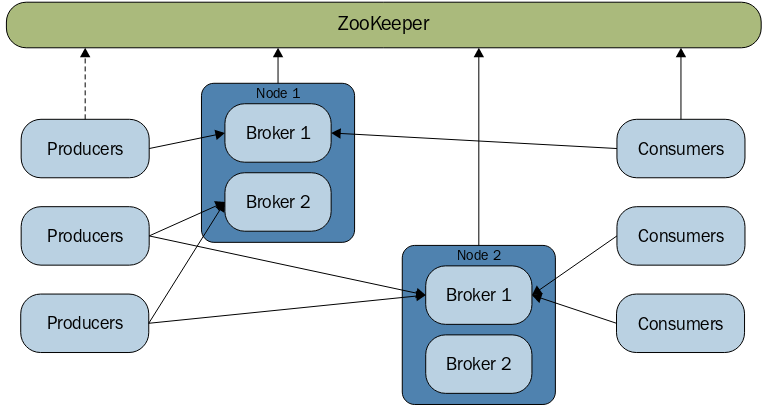
\includegraphics[keepaspectratio=true,scale=0.5]{img/kafka_multinode_multibroker}
    \caption{Multiple Broker / Multiple Node Kafka Cluster \cite{garg2013apache}}
  \label{fig:kafka_multinode_multibroker}
\end{figure}



\subsection{Mesos}
"Mesos is a cluster manager aiming for improved resource utilization by dynamically sharing resources among multiple frameworks " \cite{kakadia2015apache}.\\
The aim behind this framework is to provide a single platform which takes care of all hardware resources like CPU, memory, disk etc.
For the developer the whole cluster looks just like one big machine with cumulated resources.
This layer of abstraction makes it very easy to deploy and maintain applications running in a cluster.\\

According to mesos.apache.org \cite{apache_mesos}, there are some key features which make Mesos an attractive candidate as cluster manager for a big data stack like SMACK.
\begin{itemize}
    \item Linear scalability
        As proven by industrial application, scaling up to 10,000s of nodes is possible.
    \item High availability
        Zookeeper plays a key role when dealing with fault-tolerance, as the replicated master nodes use it to provide high availability.
        In addition it is possible to perform non-disruptive upgrades in the cluster.
    \item Containers
        Services like Docker run natively on Mesos.
    \item APIS
        There is a command-line tool to execute commands conveniently perform operations in the cluster, as well as a straight forward HTTP API to do requests programmatically.
    \item Cross Platform
        Mesos is supporting platforms like Linux, Windows, OSX and most cloud providers out of the box.
\end{itemize}

"In SMACK, Mesos orchestrates components and manages resources.
It is the secret for horizontal cluster scalation. ...
The equivalent in Hadoop is Apache Yarn" \cite{estrada2016big}.


\subsection{SMACK Stack}
Each SMACK technology for itself has proven to be robust and do an excellent job for the apsect it was designed for.
To build a big data architecture, we need frameworks which have connectors and can be easily put together to a powerful data pipeline.
Of course each of the technologies could be replaced by some other framework, but it has been shown, that those of SMACK are linkable very well \cite{estrada2016big}.\\
It is important to see, that SMACK focuses on \textit{fast data} and not necessarily only on \textit{big data}.
As the requirements of most modern large-scale applications demand processing in almost real-time, the need of such a stack is just the logical consequence.\\
"The SMACK stack emerges across verticals to help developers build applications to process fast data streams ...
The sole purpose of the SMACK stack is processing data in real time and outputting data analysis in the shortest possible time, which is usually in milliseconds" \cite{estrada2016big}.\\

Putting it together, Figure~\ref{fig:smack_stack} illustrates how the combination of Spark, Mesos, Akka, Cassandra and Spark could look like in a big data pipeline.
There are several users, endpoints or simply events which needs to be analyzed and processed.
While using Kafka producers to ingest the data, a consumer could directly be implemented in Spark using an available connector.
Storing the data in Cassandra is just a few lines of source code when using the Spark-Cassandra connector, which makes the pipeline easy to implement.
In this example the power of Akka is used to create a reactive application to give feedback to the users in a highly concurrent way and fault-tolerant by design.
Running all those frameworks on Mesos provides another layer of abstraction, so that the developer does not need to take care about the underlaying hardware and can let Mesos do its job as cluster manager.\\
This is just one of many possible setups for the stack.
The two applications used in this thesis to evaluate the results are described in more detail in Section~\ref{sec:evaluation_setup}.\\


\begin{figure}[!htbp]
  \centering
  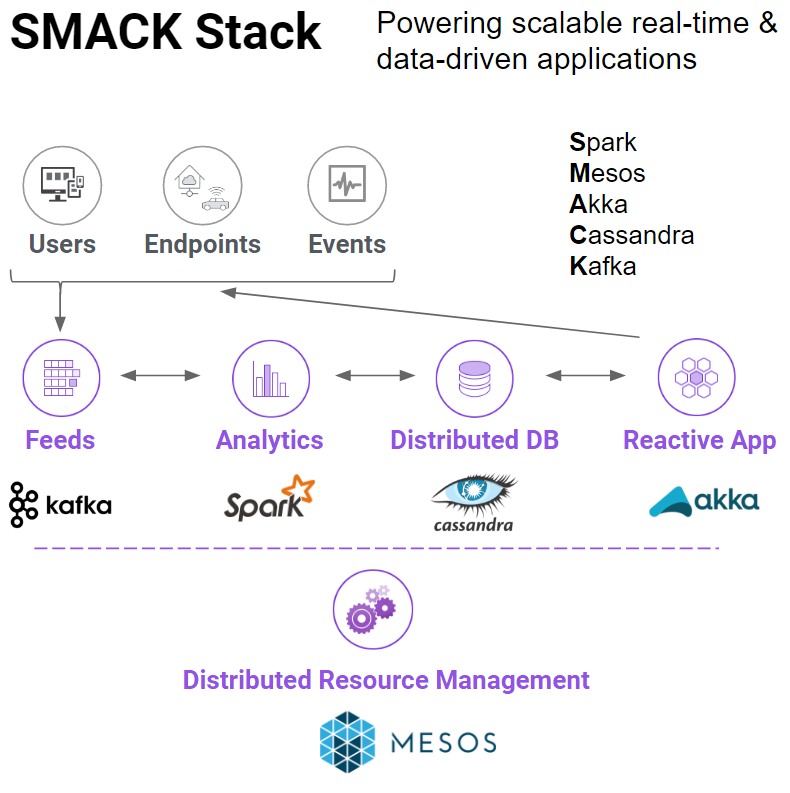
\includegraphics[keepaspectratio=true,scale=0.4]{img/smack_stack}
    \caption{SMACK Stack Illustration \cite{mesosphere}}
  \label{fig:smack_stack}
\end{figure}

\subsection{Reactive Systems}
Most modern applications have to fulfill high standards and many claim to be "reactive" systems.
The term "reactive system" is defined in the Reactive Manifesto \cite{reactive_manifesto}, where essentially four key factors have to be given to attribute an application as reactive:
\begin{enumerate}
    \item \textbf{Responsive}\\
          This attribute describes that the application has to respond in a defined time frame under all circumstances, as long as an answer can be given to the query.
          Without the definition of a time to response, it is not possible to determine whether an error occurred or not.
          Further fast response times improve user confidence and trust into the system and makes the whole application more interactive, which is highly desirable.
    \item \textbf{Resilient}\\
          Even in the event of hardware- or software faults, the system should stay intact and be able to respond to user queries.
          This is not only the case for highly critical applications but for any "reactive" system.
          The only way to achieve resilience, is to isolate components, use replication and delegate responsibilities.
          In case of an error only an isolated subsystem is affected and the supervising platform can recover this faulty component without affecting the whole application.
    \item \textbf{Elastic}\\
          Systems which are elastic stay responsive even under varying load.
          This means that the application can react to an increasing number of requests and still provide the required functionality even during peaks.
          The base for elasticity are these two key factors: replication and distribution of functionality.
          Elasticity also describes that if there are less requests than expected, the system can scale down and release resources which are not needed at the moment.
    \item \textbf{Message driven}\\
          The use of asynchronous messages is crucial to allow loose coupling and isolation of different components.
          The non-blocking nature of these messages lead to an efficient use of resources, as any component which is not receiving messages can stay idle and therefore does not consume CPU time.
          Further the explicit use of a message driven architecture allows to be independent of the location, as well as transparent scaling of components.
\end{enumerate}
The applications used in this thesis to evaluate strategies and the developed framework are reactive systems, which meet the criteria defined above.


\section{Thesis Organization}
In chapter \ref{ch:related}, related work can be found, including the comparison and summary of existing approaches.\\
Chapter \ref{ch:implementation} deals with the framework developed in the context of the thesis, including all its components.
Additionally there is an architecture overview, as well as the deployment diagram is discussed.
To give a deeper understanding of what is considered "interesting" for the framework when deciding which component to scale, the relevant metrics for each technology are discussed.
In chapter \ref{ch:evaluation} the evaluation and interpretation of the benchmark results can be found.
The experiment setup for the benchmark is described, including challenges and restrictions.
To give the reader a better understanding of the benchmark, a section about evaluation criteria and one about the significance of the benchmark is added to the chapter.
Further the setup, i.e. the applications used for the evaluation and the target architecture are described in this chapter.\\
The last chapter, \ref{ch:conclusion}, is about open issues, the conclusion itself and possible future work.

\section{Methodology}
The scientific approach used in this thesis comprises six parts.\\
In the first step, a literature review is performed and background information has to be gathered to serve as the theoretical background for this work, building on existing research.
After that an important part is the technology exploration.
In this step the individual parts of the SMACK-Stack have to be explored and knowledge about each technology is gathered.
In addition technical literature and reference books about the respective technologies can be read to get a better overview and a deeper understanding of each part of the SMACK stack.\\
The next step is the cloud setup, in which he whole stack is configured to be easily deployed.
One tool could be Amazon CloudFormation to provide a simple template for launching preconfigured instances.
Further various scripts have to be written to automate the deployment process an install required libraries, scripts and later on the applications to evaluate.\\
In the next step - the development - the framework to automatically redistribute and elastically scale the resources is implemented.
Further the two real world applications for the experiment benchmarks are implemented and extended to fit the needs of this thesis.
During the next step, namely the experiments, the scalability of the stack is determined by benchmarking individual configurations, where one application uses real world IoT data.\\
Then the performance of the stack under management of the developed framework is examined carefully.\\
In the last step the results are interpreted and the suggestions for how to distribute the resources are deduced and the corresponding reference deployment architecture and configuration is defined.


%%%%%%%% CHAPTER %%%%%%%%%
\chapter{Related Work}
\label{ch:related}

\section{Literature Studies}
Currently, there exists no specific suggestions on how to optimally use the SMACK-stack in the aspect of resource distribution between the individual technologies.
Further this thesis focuses on the scalability of the whole stack and aims to find bottlenecks when dealing with various input data patterns.
There is research for each of the technologies but not in their combination, and especially there are no recommendations based on empirical experiments for how to setup the stack optimally with a given budget and specific requirements.

\subsection{Cloud Computing \& Big Data}
There is a lot of research in the field of cloud computing and big data.
In their paper "Fast Data in the Era of Big Data" Mishne et al. show the background of Twitters new spelling correction and query suggestion, which has the demand to include recent events within minutes \cite{mishne2013fast}.
The approach shows that the commonly used Hadoop-based approach did not work out well, as the provided latency was simply to high.
In the final result they build their own in-memory processing engine, to be able to handle data faster.
This is similar to Apache Spark, as it also works in-memory and claims to be faster than traditional Hadoop based approaches.\\

Agrawal et al. provide an overview about basic design decisions concerning scalable cloud applications and point out actual problems and open questions \cite{agrawal2011big}.
They provide a study which comprises two types of systems: 1) write-intensive applications, such as large DBMS systems and 2) systems which provide ad-hoc analysis, where the focus lies on speed and low latency.
In the paper there are some suggestions in form of design choices, based on successful large systems in the field.\\
In the work of Hashem et al. the current development of big data as phenomena and its challenges, as well as open research issues are discussed \cite{hashem2015rise}.
Cloud computing is designated as powerful tool for many applications, when it comes down to handle huge amounts of data and scalability is a key factor.
Further it is stated, that cloud computing enabled the rise of big data in the first place, as elasticity and scalability is relatively easy to achieve compared to on-premise setups.
The definitions, classifications and typical characteristics of such applications are explained and introduced.
In the end, the authors illustrate open research issues and show further fields of research.\\
In the article of Armbrust et al. about cloud computing it is stated that it "has the potential to transform a large part of the IT industry, making software even more attractive as a service and shaping the way IT hardware is designed and purchased" \cite{armbrust2010view}.
The authors give an overview of what cloud computing is and what to challenges to face.
In the conclusion they discuss the potential of modern technologies and give an outlook for future applications.\\
To be able to compare the pros and contras of existing cloud computing providers, Rimal et al. investigated on the taxonomy of the different providers and then compared them in aspects of architecture and services.
The output of their comparison is a table with generic attributes such as computing architecture, virtualization management, load balancing, etc.
In the conclusion, the authors state that "Cloud Computing is the promising paradigm for delivering IT services as computing utilities" \cite{rimal2009taxonomy}.\\

With their work "Big Data: The Management Revolution", McAfee and Brynjolfsson explain why a new way of thinking in modern businesses is crucial \cite{mcafee2012big}.
They state that "using big data enables managers to decide on the basis of evidence rather than intuition.
For that reason it has the potential to revolutionize management" \cite{mcafee2012big}.
Explanations about how the shift of data driven management can be revolutionary are given, and the core properties of big data, which are the three Vs (Volume, Velocity, Variety), are discussed.
Further, a simple four step getting started guideline, as well as five management challenges are illustrated to enable readers to apply the introduced values to their own business management.\\

\subsection{SMACK Stack}
In the book "Big Data SMACK" of Estrada and Ruiz, Apache Spark, Mesos, Akka, Cassandra and Kafka are motivated and explained \cite{estrada2016big}.
The book gives a good introduction of why this stack is crucial for the success of many modern business applications and shows how to combine the individual technologies to a powerful data pipeline for fast data applications.
As the book offers an overview, the authors are not going into detail and scalability is just mentioned but never proved.\\

In their whitepaper "Fast Data: Big Data Evolved", Wampler and Dean present an overview of how business changes and so do technology in the field of big data \cite{wampler2016fast}.
The term \textit{Fast Data} is introduced to be the logical consequence of the big data requirements plus the need of near- or real time applications.
The authors list key components and technologies of a modern fast data application, which contain - not surprisingly - Scala, Akka, Spark, Cassandra, Mesos, Docker and Kafka.
SMACK contains the same technologies and in this thesis also Docker is used, which reflects the power of the combination of these technologies when working together as big data / fast data pipeline.\\


\subsection{Big Data Frameworks}
The paper of Zaharia et al. from the University of California introduces the Spark framework for the first time \cite{zaharia2010spark}.
Spark's structure and advantages over traditional Hadoop-based applications is shown and demonstrated.
There are experiments which show, that most machine learning algorithms Spark outperforms Hadoop by up to 10 times, which is a lot.
Especially the in-memory data handling speeds up the whole process dramatically.
The numbers and experimental data from this paper could be a base for further research in this thesis, but still it only benchmarks one technology and not a whole stack.\\
A further article shows how important the development of a computation framework for the increasingly huge amounts of data has become \cite{zaharia2016apache}.
In their work the authors show how Apache spark serves as unified data processing engine in the field of big data analytics.
They compare the performance to existing and common Hadoop implementations, which are significantly slower when it comes to iteration within the algorithm.
This can be explained with the fact that Hadoop is disk base, while Spark tries to manage its data structures in-memory and can therefore be dramatically faster.
The conclusion appeals to Apache Spark to encourage more open source frameworks to be interoperable with it and to make the use of complex software compositions even easier.\\

To go more into detail about the commonly discussed Hadoop vs. Spark topic, the paper of Gu and Li gives insights about the question memory vs. time \cite{gu2013memory}.
As Spark relies by design heavily on in-memory operations, Hadoop is disk-based and thus, iterative algorithms can be performed significantly faster with spark, as the costs of reloading and caching data are lower.
Therefore more memory is required, which is a cost critical factor when designing the system architecture.
Further they show, that as soon as there is not enough memory available to store intermediate results, Spark slows down.\\

To emphasize the importance of Apache Spark in the field of cloud computing, the paper of Reyes et al. compare it to OpenMP by performing big data analytics \cite{reyes2015big}.
The motivation behind the experiment is that handling vast amount of data in parallel is still a challenge when dealing with near-time or even real-time applications.
For the evaluation, two machine learning algorithms, both supervised, are used in the Google Cloud Platform.
Data management infrastructure and the ability to provide fault tolerance out of the box is where Apache Spark did a better job, although the performance of the OpenMP implementation is more consistent in terms of processing speed.\\

As this thesis deals with the NoSQL database management system Cassandra, the survey on NoSQL databases of Han et al. has its relevance \cite{han2011survey}.
In the introduction the authors give an overview of which characteristics and requirements a modern NoSQL system has to fulfill.
By walking through the CAP Theorem (Consistency, Availability and Partition tolerance) they show what is possible and what not for a system as Cassandra.
They try to classify existing solutions into key-value and column-oriented databases.
Further some existing systems are summarized and their core values are emphasized.\\

Just as Cassandra, Kafka plays an important role in the SMACK stack.
The paper of Kreps et al. from LinkedIn introduce Kafka as "a distributed messaging system for log processing" \cite{kreps2011kafka}.
Initially Kafka was designed to handle vast amounts of log files, but as the authors show, the system is also capable of handling other message based applications very well.
First the framework itself is illustrated and the architecture as well as some design principles are discussed.
The authors give an insight of how they use Kafka at LinkedIn and why they choose its design as it is.
In the results section, Kafka is compared to existing enterprise messaging systems such as activemq and rabbitmq, where their framework significantly outperforms the others.\\

DCOS, the Data Center Operating System of Mesosphere, is used in the context of this thesis to setup and manage the SMACK stack.
Therefore the paper of Hofmeijer et al. is relevant as they introduce this platform and give insights about the internal structure \cite{hofmeijer2004dcos}.
The power of DCOS is to provide a layer of abstraction to the system resources in a distributed cluster.
Further the availability of software packages leverages the usually complicated task of deploying a frame work like Apache Spark in production mode in the cluster.\\

\subsection{Streaming}
As streams play a key role in Spark as well as in big data, the paper of Namiot about "Big Data Stream Processing" is also relevant for this thesis \cite{namiot2015big}.
In his work, Namiot gives an overview of existing technical solutions for stream processing with big data.
He also mentions IoT, which is often the main source of input data for cloud applications and may be relevant for the experimental setups in the thesis.
Further, Spark is mentioned too and explained in more detail.\\

Another streaming relevant work is the article of Ranjan about "Streaming Big Data Processing in Datacenter Clouds" \cite{ranjan2014streaming}.
He describes the motivation behind the topic and illustrates a data pipeline for large-scala data processing in the cloud, which is similar to SMACK, but less complex.
"The example service consists of Apache Kafka (data ingestion layer), Apache Storm (data analytics layer), and Apache Cassandra Systems (data storage layer)" \cite{ranjan2014streaming}.
The listings in this article may be relevant for arguing why to use Apache Spark over Apache Storm for example.\\


\subsection{Languages \& Programming Models}
The actor model is the mathematical theory behind Akka and is widely known to be efficient for building parallel applications.
P. Haller from Typesafe Inc. gives an overview "on the integration of the actor model in mainstream technologies" \cite{haller2012integration}.
The knowledge of this model is important in the context of this thesis as Akka is the de-facto standard implementation of the actor model and there are some design principles to consider when designing a highly concurrent application with this mathematical model as base.
The author states that there are some challenges for the implementation of such framework into existing platforms as the JVM, because it is not designed to handle concurrency this way.
Those fundermental problems are illustrated and possible solutions are suggested, while the focus lies on the Scala programming language, which is heavily used in this field due to its functional nature.
In the paper the requirements of a well designed actor implementation is discussed and based on that, "principles behind the design and implementation of actors in Scala are explained, covering (a) the programming interface, and (b) the actor runtime" \cite{haller2012integration}.\\
Tasharofi et al. investigate in their paper why Scala developers ofteh mix conventional concurrency models with the actor model \cite{tasharofi2013scala}.
The use of a mix causes that the actor model is no longer consistend and can cause race conditions or leverage the benefits of using it at all.
About 80\% of the investigated publicly available frameworks are using a mix between at least two concurrency models.
The finding of the authors is that often this mix is choosen due to "inadequacies of the actor libraries and the actor model itself" \cite{tasharofi2013scala}.\\


\subsection{Data Analytics}
The paper of Cuzzocrea et al. about "Analytics over Large-Scale Multidimensional Data" provides an overview of actual research issues and challenges in the field of big data \cite{cuzzocrea2011analytics}.
The authors go into detail how to deal with especially multidimensional data and propose a few novel research trends.
Further data warehousing is discussed as a trend, which is relevant for big data applications in general but not especially for this thesis, as SMACK usually handles data streams where queries usually require a quick response time.
Still the analytical part of the paper is interesting in this context.\\

The white paper "Big Data Analytics" of P. Russom illustrates the understanding of what big data and big data analytics are and what it means for modern a business \cite{russom2011big}.
First an extensive introduction shows what exactly big data is and also gives an idea of how most people in the field see the technology.
In the survey explicitly the question of how familiar people are with big data analysis, is discussed.
The common understanding is quite well, but based on the given 325 interviewed candidates only 28\% said they really know what it means and can correctly name it.
In addition the benefits of such a technology are listed, where the most popular answer, with 61\%, is a "better targeted social influencer marketing" \cite{russom2011big}, and "more numerous and accurate business insights" \cite{russom2011big} is with 45\% on the second place.
The conclusion gives a pretty compact list of recommendations to follow when dealing with big data and big data analysis.\\


\section{Comparison and Summary of Existing Approaches}
This section gives an overview of existing tools and approaches to solve the problem of automatically scaling the SMACK stack or similar technologies in the cloud.\\

The problem of how to realize "Efficient Autoscaling in the Cloud Using Predictive Models for Workload Forecasting" is covered in the paper of Roy et al. \cite{roy2011efficient}.
The autors contribute in three aspects to this challenge.
At first a discussion of current challenges in the field of cloud computing and autoscaling is given.
Second, the developed algorithm to forecast work load is introduced, which is later investigated in terms of performance by conducting empirical experiments.
Their algorithm works fine for constanly increasing or alternating workloads, but suffers from unexpected peaks.\\
Compared to the framework developed in this thesis, Roy et al. provide an algorithm rather than a framework to implement autoscaling.
Further the consideration of multiple metrics is missing, as they only consider the incoming workload instead of monitoring each component individually.
Still a combination of the predictive and the reactive approach would be possible and could be subject of future work.\\

The paper "Dynamic Scaling of Web Applications in a Virtualized Cloud Computing Environment" of Chieu et al. introduces a novel architecture \cite{chieu2009dynamic}.
In their main contribution, the autors illustrate a "front-end load-balancer for routing and balancing user requests to web applications" \cite{chieu2009dynamic}.
The use of load-balancer can help to provide more reliable web-services and reduce costs too.
As the approach only covers scaling based on user requests, on the one hand this solution cannot react on internal stress, for example caused by a computational intense Spark job, which is implemented in the framework of this thesis on the other hand.\\

\textbf{Mesosphere Marathon-Autoscale} \cite{marathon_autoscale}\\
This tool is a python script which is deployed within a Docker container on DC/OS and interacts with Marathon.
The information about the CPU and RAM usage is gathered by asking directly Marathon and in case a certain threshold is reached, the Marathon API is used to scale up the service.
In the same way the down scaling is implemented.
Some configuration is possible, such as defining the desired thresholds and the services to observe.\\
This is a very basic approach, as only the CPU and RAM usage is considered, which is a fuzzy indicator for the real utilization of the service.
With only this information it is not possible to reliably determine whether a service will be out of resources soon or not, especially when dealing with complex applications, such as the ones in the SMACK stack.\\

\textbf{Mesosphere Marathon-LB-Autoscale} \cite {marathon_lb_autoscale}\\
With this tool the High Availability (HA) Load Balancer (LB) is used to determine which service is under heavy load and needs to be scaled up.
In Figure~\ref{fig:marathon_lb_autoscale} the architecture of the tool is illustrated.
It works by analyzing all incoming traffic via the HA proxy, which load balances the data between the service instances inside the stack.
Therefore it is possible to see how many requests per second each service and instance has to handle.
On the base of those statistics, the tool then uses the Marathon API to scale up or down a service.\\
This tool also comes within a Docker container, which makes it easy to deploy it on DC/OS.
Still there is some configuration effort, such as defining the URLs for the HA proxy and Marathon, sampling rate, thresholds etc.
This approach is useful for TCP traffic based services but cannot handle all services in the SMACK stack as there is usually just one service responsible for handling incoming data from the internet.
In contrast, the framework developed in the course of this thesis is capable of extracting metrics for all relevant parts of the cluster and scaling them accordingly, regardless whether they are TCP based or not.

\begin{figure}[!htbp]
  \centering
  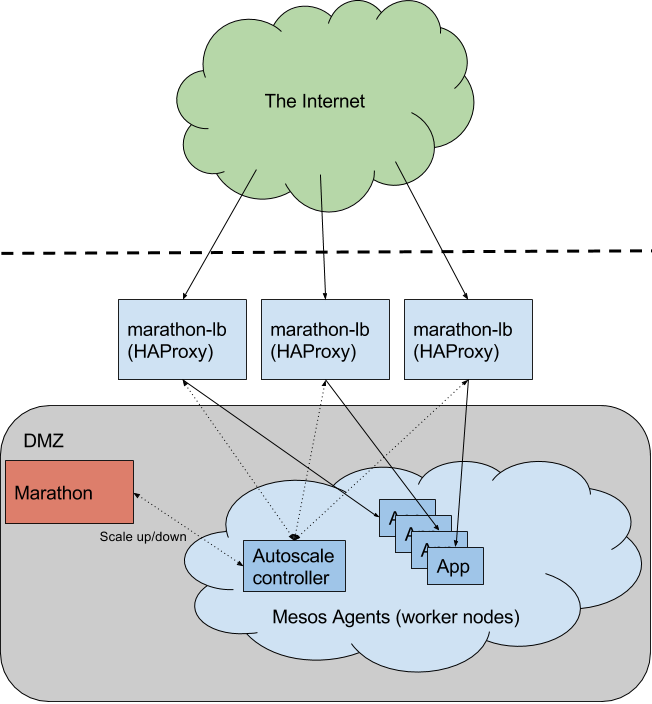
\includegraphics[keepaspectratio=true,scale=0.3]{img/marathon_lb_autoscale}
    \caption{Marathon LB Autoscale Architecture \cite{marathon_lb_autoscale}}
    \label{fig:marathon_lb_autoscale}
\end{figure}

\textbf{Microscaling in a Box} \cite {microscaling}\\
This service is one of many micro scaling implementations and provided by \textit{microscaling systems}.
It works by transferring the data between the applications via their own queue.
Then a target length can be defined which the tool tries to sustain then, which means it scales up or down a service based on the queue length.
The only metric supported is this queuing technique, which additionally takes advantage of the fact that launching further Docker container is relatively fast in comparison to launching an additional VM instance.
This is why the company claims to "automate scaling in real time" \cite{microscaling}.\\
The approach is suitable for services where the performance and workload mainly correlates with the incoming amount of data.
This is not the case in the whole SMACK stack, for example Spark could be overloaded with just a few messages in a computational bound application.
Further the usage of an additional queue between all services would slow down the stack and consume CPU and RAM resources.\\

None of the introduced tools or frameworks have a deeper look insight the SMACK stack to be able to tell whether or not a service is really under heavy load.
Those tools could be combined to get more insights but would therefore also consume a lot more resources, which is not desirable at all.
To be able to accurately monitor Akka for example, custom metrics have to be considered, which is very unlikely to be found in a generic autoscale tool.\\
The framework develped in the course of this thesis enables users to benefit from a deeper understanding of the components running in the SMACK stack to reliably detect when a service needs to be scaled.
This is done while being independent from TCP traffic based measurements or queue-length based approaches.
Further the framework is capable of handling user-defined metrics and is robust, as it can be hosted outside the cluster containing the SMACK stack.


%%%%%%%% CHAPTER %%%%%%%%%
\chapter{A Framework for Automated Monitoring and Scaling of the SMACK Stack}
\label{ch:implementation}

This section gives a detailed view of the actual contribution in the scope of this thesis.
The developed applications, stress tests and tools are introduced and their architecture is illustrated.
To review the code, there is a public git repository containing the implementations mentioned in this chapter \footnote{https://bitbucket.org/B3n3/smack}.\\
For the development mainly the Java programming language was chosen, as it is platform independent and appeals a broad audience.

\section{The SMACK Monitoring Metrics and Elasticity Actions}
As part of the theoretical background, this section gives an overview of which metrics are considered as interesting for the context of this thesis.\\

\subsection{Kafka}
In the official DataDog Github repository there is a documentation of which metrics can be interesting when analyzing Kafka via JMX \cite{datadog_kafka}.
Those proposed metrics were considered and then refined by empirical experiments to find out which ones are good indicators when Kafka is under heavy load.\\
In Table~\ref{tab:jmx_kafka} the metrics considered in this thesis concerning Kafka monitoring are illustrated in detail.

\subsection{Cassandra}
DataDog also provides an introduction to Cassandra monitoring and emphasized which JMX values to investigate when monitoring a cluster \cite{datadog_cassandra}.
Like for the Kafka metrics, those presented MBeans were refined during empirical experiments.
In Table~\ref{tab:jmx_cassandra} all relevant Cassandra JMX metrics are listed and described.

\subsection{Spark}
During the analysis of the IoT application introduced earlier, all available JMX metrics are collected.
The script to extract the Spark JMX values of Section~\ref{sec:jmx_extract_tool} filters out everything which is not directly related to the driver running in Spark.
This is done by applying a regular expression as matching criteria, which looks like this: \verb"KafkaToCassandra|.driver", where \textit{KafkaToCassandra} is the Spark driver name in the IoT application.
The regular expression considers everything which is either part of the custom class or the driver itself.\\
It is necessary to use this approach, as the MBean names exposed by Spark contain IDs which change every time the driver is launched.
An example for such a name could be this: \textit{metrics:name=43f6de33-9485-4bbe-8dbf-263b62d2a15a-0005-driver-20170731143634-0001.driver.DAGScheduler.messageProcessingTime}.\\
By analyzing the plots of the collected metrics, the ones described in Table~\ref{tab:jmx_spark} are considered most interesting.

\subsection{Akka}
As mentioned in Section~\ref{sec:jmx_extract_tool}, Akka does not provide JMX metrics out of the box.
It is up to the developer to collect metrics and then implement the exposure of them.
In the course of the contribution of this thesis, those features are implemented.\\

Fortunately there is an open-source project to ease the task of exposing JMX values.
The framework is called \textit{Kamon}, which "is distributed as a core module with all the metric recording and trace manipulation APIs and optional modules that provide bytecode instrumentation and/or reporting capabilities" \cite{kamon}.\\
In addition there are two dedicated Akka modules in Kamon, which expose some useful default metrics.
To be able grab and expose JMX values from an existing application, AspectJ Weaver is used.
It is a non-trivial task to handle all required dependencies and correctly launch the application with AspectJ in a Docker container.
Setting up things require knowledge in the field of virtualisation with Docker and dependency management.\\

In addition to the already by Kamon provided metrics, \textit{KB/s} and \textit{Messages/s} are added to give more flexibility when monitoring the application.
In Table~\ref{tab:jmx_akka}, all considered metrics are illustrated and described in detail.


\subsection{Mesos}
As there is no possibility to enlarge RAM or CPU resources for Mesos and because it is the underlying system, there is no need to monitor it explicitly in the context of this thesis.


\section{Framework for Automated Monitoring and Scaling}
This section introduces the framework developed in the course of this thesis.
First there is an architecture overview to better understand how the respective components interact.
Secondly the respective components and tools are illustrated and explained in detail.

\subsection{Framework Architecture Overview}
In this section, an overview of the framework is given, including architecture and deployment diagrams.

\begin{itemize}
    \item \textbf{Automated Scaling Tool for SMACK}\\
          The scaling tool evaluates the collected metrics from the REST service and scales up or down the individual parts of the SMACK stack.
    \item \textbf{REST Service Collecting Monitoring Information}\\
          This is the service which collects all the extracted metrics and compiles them into a useful format.
          In addition there is the possibility to generate plots at runtime.
    \item \textbf{JMX Extraction Tool}\\
          This tool is designed to automatically extract interesting metrics from SMACK components via JMX and sending them to a central service, in this case the REST monitoring service.
    \item \textbf{Framework to Easily Launch SMACK in AWS}\\
          With the help of this framework it takes just a few command line calls to launch and deploy the whole SMACK stack in the cloud.
    \item \textbf{Deployment Blueprints}\\
          Those reference architecture and configuration recommendations help to launch the SMACK stack and getting most out of the available resource.
\end{itemize}

Figure~\ref{fig:architecture} illustrates the target architecture of the framework and how the tools and services interact with each other, while Figure~\ref{fig:overall_view} shows the deployment view.\\
The SMACK stack is the central element in this architecture and is illustrated by many AWS EC2 instances working together as one stack.
In the same environment - namely DC/OS - the JMX Extraction tool is running in Docker containers, collecting metric statistics from the SMACK stack.
For each node, or EC2 instance, there is exactly one Docker container started and associated.
The container runs on the same instance to be able to access the JMX values from the available services.\\

In case there is no service deployed on the node, the JMX extraction tool is idle and automatically starts extracting as a service gets deployed.\\
To launch and setup DC/OS the Cloud Formation tool of AWS is used, which manages the complex installation of all required components and glues them together automatically.\\
The extracted metric values are directly send to the REST monitoring service, which runs on its own dedicated EC2 instance totally independent of the DC/OS setup.
There the information is collected and combined to be evaluated later.\\

If it is the case that the IOT application is running in the SMACK stack, the load generator introduced in section \ref{sec:load_generator} is also part of the setup.
As described, the AWS EC2 Container Service is used to easily orchestrate the execution of multiple docker images performing the requests.
ECS enables to simply de- or increase the amount of running Docker containers and is also independent of the DC/OS setup.
There is no information flow from DC/OS to the load generator.\\

All previously described parts of the setup are running in the AWS cloud.
The only application running on a local machine is the scaling tool itself.
By querying the REST monitor, the scaling tool gets up-to-date information about the workload of the SMACK stack.
In case the stack get's offline or does not respond in time, the monitoring service is still responsive because it is completely decoupled from the rest of the stack.
The user interacts with the scaling tool which in turn interacts directly with DC/OS to manipulate the SMACK stack in case a component needs to be scaled up or down.

\begin{figure}[!htbp]
  \centering
  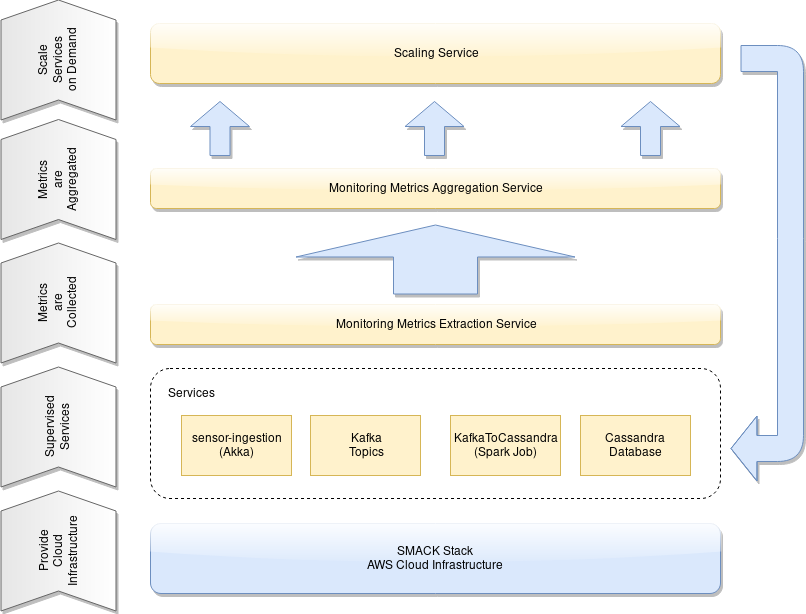
\includegraphics[keepaspectratio=true,scale=0.55]{img/architecture}
    \caption{Framework Target Architecture}
    \label{fig:architecture}
\end{figure}

\begin{figure}[!htbp]
  \centering
  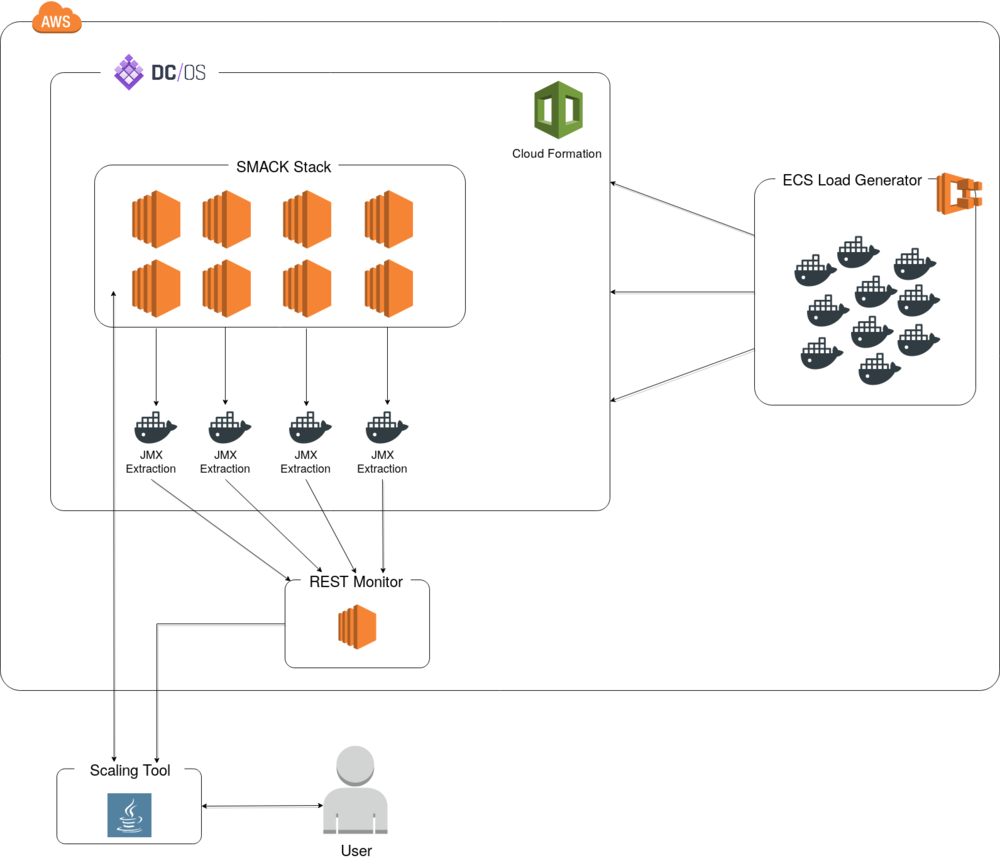
\includegraphics[keepaspectratio=true,scale=0.47]{img/overall_view}
    \caption{Framework Deployment View}
    \label{fig:overall_view}
\end{figure}



\subsection{Monitoring Metrics Extraction Service}
\label{sec:jmx_extract_tool}

To be able to monitor each SMACK component individually, considering more than just plain RAM and CPU usage, a more sophisticated approach is required than only observing the provided DC/OS usage metrics.\\
First we will have a look on the technical aspect of how to gather information and then why the proposed approach was chosen.\\

Collecting runtime information from an application is a common task and there are some well-known ways to do so.
Webservices for example, often provide a REST API to access internal status information.
As the applications used in this thesis all run in the Java Virtual Machine (JVM), it is possible to use the Java Management Extensions (JMX) as information channel.\\
This is especially useful as Kafka, Cassandra and Spark are configurable to publish monitoring statistics via JMX without any extra programming.
Akka is not able by default to export to JMX which means all the steps - form acquiring the statistical data to publishing them - have to be programmed into the Akka application.\\

Figure~\ref{fig:jmx} shows the basic architecture of JMX.
The distributed services level, serves as entry point to access the interface.
There is no defined specification and the purpose is to provide a way to communicate with the deeper agent level.\\
Through the interface the client is able to access the agent level, where the agents reside and are responsible for the communication with the instrumentation level.
In the last level, the real resources can be found, which are managed and configured with the so called \textit{Managed Beans (MBeans)}.\\
With the help of MBeans it is possible for an application to expose values through JMX, which can then be read by a client via the JMX interface.\\

\begin{figure}[!htbp]
  \centering
  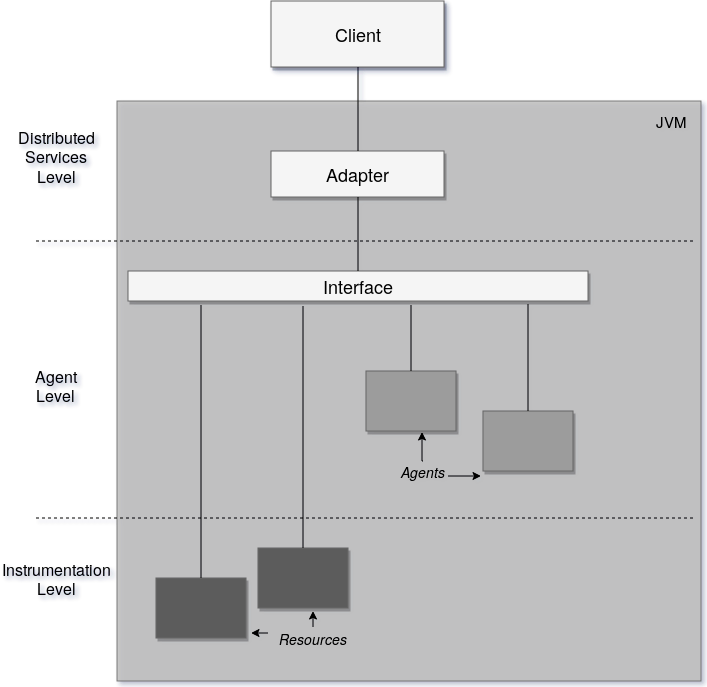
\includegraphics[keepaspectratio=true,scale=0.45]{img/jmx}
    \caption{JMX Architecture Overview}
  \label{fig:jmx}
\end{figure}

In order to access JMX MBean values of running JVM instances, there are some open source tools available.
JConsole is a graphical tool which ships with the JDK and allows the user to get an overview of a running system.
However, this tool requires a GUI, and does not provide an API to use it with scripts or via command line.\\
An open-source tool, which offers this interface is Jmxterm.
"Jmxterm is a command line based interactive JMX client.
It's designed to allow user to access a Java MBean server in command line without graphical environment.
In another word, it's a command line based jconsole" \cite{jmxterm}.\\
MBeans contain attributes which could be \textit{Value}, \textit{OneMinuteRate}, \textit{Mean}, \textit{Count} and so on.
As part of the contribution of this thesis, a script to automatically extract the desired MBean values and send them to a monitoring service is provided.
The abstract algorithm of the script can be described as follows:

\begin{enumerate}
    \item Get the current timestamp.
    \label{enum:current}
    \item Read the provided JMX commands from the input file.
    \item Create a list of all occurring MBeans in the given file.\\
        This list is needed, as the output of Jmxterm does not contain the name of the MBean itself.
    \item Open the CSV output file and add a column header if the file is empty.
    \item Execute Jmxterm with the provided command file and split the output lines by newline.
    \item For each line:
        \begin{enumerate}
            \item Extract the attribute name and the respective value of the output.
            \item Write the data into the CSV file.
            \item Send the data to the given REST monitoring service via HTTP POST.
        \end{enumerate}
    \item Close all files and sleep for a given period of time.
    \item Go to \ref{enum:current}.
\end{enumerate}

The exported values of the script are: \textit{Timestamp}, \textit{MBean name}, \textit{Attribute name}, \textit{Value} and \textit{Hostname}.\\
The hostname is important, as it is the only way to distinguish from which node the value comes from.
In addition it is required to later on generate statistics and accumulate the value of the same MBean-Attribute combination across different nodes.\\
The script works fine for a static input file, which means the names of the MBeans are known in advance and do not change during the analysis.
However, Spark exposes MBeans which contain the ID of the worker node or the task number.
This makes it impossible to predefine a list of MBean names which the script should observe and send to the monitoring service.
Because of this problem, another script is implemented to extract interesting MBean names from Sparks JMX view.\\
An abstract overview of how the script works could be the following:

\begin{enumerate}
    \item Open the connection to Sparks JMX.
    \item Store all available MBeans inclusive their attributes in a list.
    \item Go through the list and filter out only interesting ones (with a regular expression).
    \item Extract the name of the attributes to the respective MBean.
    \item Store the Jmxterm commands to get the values of an MBean attribute into a command file.
\end{enumerate}

In order to be able to automatically generate new Spark command files during runtime, the script is executed regularly by the JMX extraction script.
This enables the setup to simply launch the extractor without having to deal with the manual extraction of interesting Spark MBeans and the command file generation.\\
To be able to easily deploy and manage the JMX extraction on all nodes of the cluster, the script is packed into a Docker container.
The Docker file and the respective configurations are also part of the contribution.\\

The choice to use JMX as information channel is made because of the fact, that all Spark, Kafka and Cassandra offer JMX metrics out-of-the-box.
Further it is a standardized way to access runtime information of a JVM application.
Additionally, the existence of open-source tools like Jmxterm helps to reduce manual programming effort.



\subsection{Monitoring Metrics Aggregation Service}
In order to collect the extracted JMX metrics from the particular nodes, a central point to store and access this information is needed.\\
As part of the contribution of this thesis, a REST web service running in a Docker container is implemented, which is capable of storing, collecting and exporting the metrics of the respective services.
Further it is possible to generate and view SVG plots with this service.\\

The structure of the REST service API is illustrated in Table~\ref{tab:rest} and gives an overview of the available operations.
The service is implemented using the Java programming language and runs in Docker.
This allows the monitor to be launched on different platforms easily without any configuration or setup effort.
In the context of this thesis AWS EC2 is used to host the service.\\
As part of the contribution of this thesis a CloudFormation template is created to allow the user to launch and instantiate the monitoring service in the cloud with just a few clicks.\\

To get an impression of how the service looks internally, Figure~\ref{fig:smack_rest_monitor_uml} shows the implementation of the service in an UML diagram.
The \verb|SmackRestMonitor| contains the \verb|main| method and creates all needed instances of the particular service handlers.
While the abstract class \verb|RESTHandler| already provides most of the generic business logic to handle incoming requests, the four extended classes \verb|Akka|, \verb|Cassandra|, \verb|Kafka| and \verb|Spark| only provide methods required for displaying information about the service.\\
\verb|DateValueHostname| is the central unit of stored information.
It is, as the name suggests, a tuple of the date, the senders hostname and the value of the processed request.
During the constructing the date and the value is parsed for later analysis.
The association between MBeans, attributes and those tuples is managed by the instances of the \verb|RESTHandler|.\\
To be able to calculate information like the 60 seconds maximum, average etc. (detailed information can be found in Table~\ref{tab:rest}), an instance of \verb|ValueCalculator| is created by the \verb|RESTHandler| each time a new request is processed.
This class contains the implementation and logic to calculate the requested statistical values.\\

Further, there is the option to generate SVG plots, which is done internally by using the pygal framework.
The plots are generated per MBean and contains all recorded values for all available attributes.
An example could be the message processing time which then shows the Min, Max and OneMinuteRate.
In addition to this separation, the script is are aware of multiple hosts, which is handled in three different ways:
\begin{enumerate}
      \item A separate curve for each node and attribute combination.\\
            E.g. OneMinuteRate-host1, OneMinuteRate-host2, ...
      \item The average of all hosts for the same attribute.
      \item The sum of the values of all hosts for the same attribute.
\end{enumerate}
In case two and three, a sliding time window is used to find corresponding entries.
This is required as the data needs to be aligned somehow on the time line.

\begin{figure}[!htbp]
  \centering
  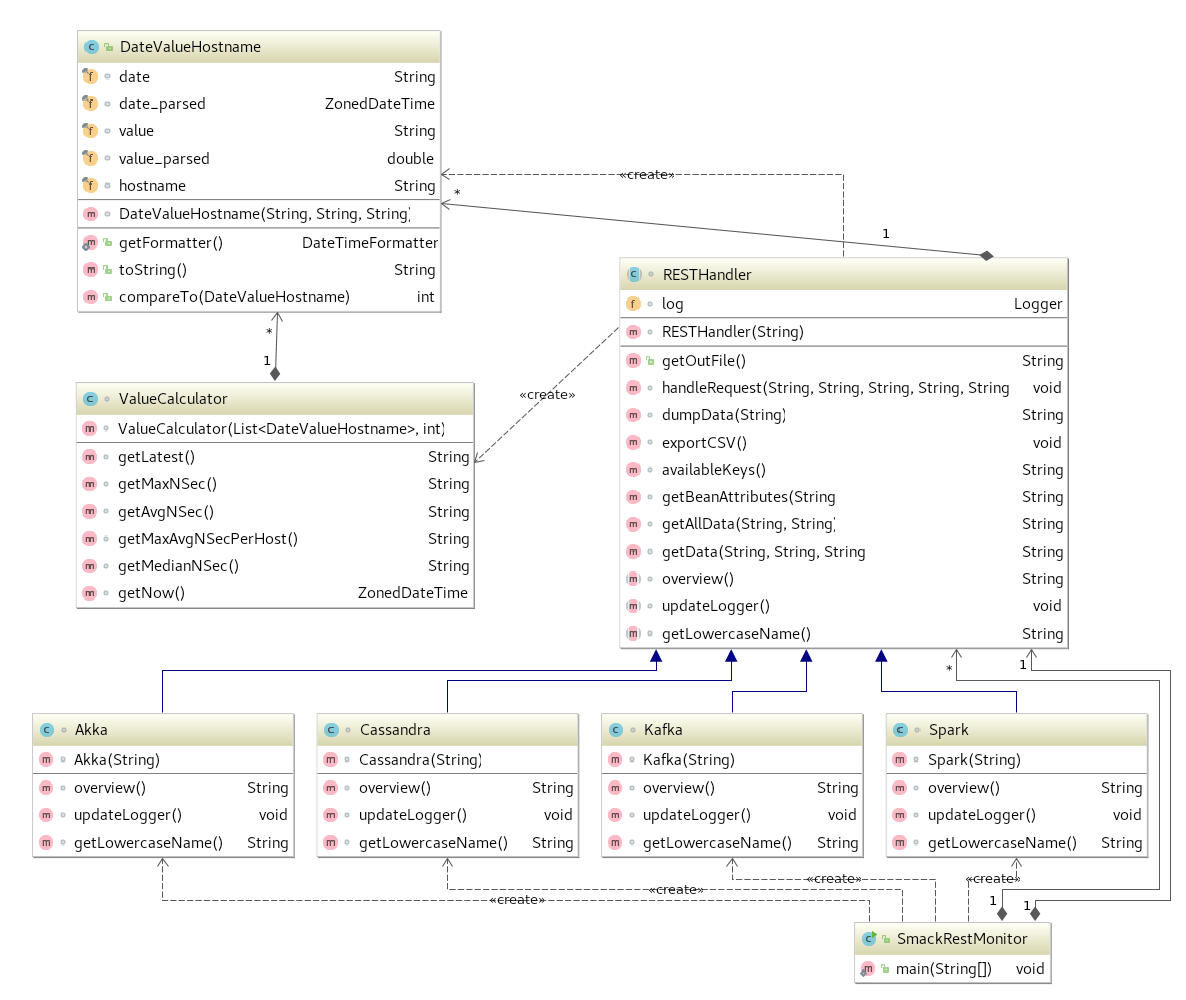
\includegraphics[keepaspectratio=true,scale=0.42]{img/smack_rest_monitor_uml}
    \caption{SMACK REST Monitoring Service}
  \label{fig:smack_rest_monitor_uml}
\end{figure}

\begin{table}[]
\setlength{\extrarowheight}{.5em}
\begin{tabular}{@{}lp{8cm}@{}}
\toprule
URL & Description \\ \midrule
/                                       & Displays an overview page with links to the particular services and available operations.  \\
/<service>                              & Overview page of the respective service which contains links to further operations. \\
/<service>/dump                         & Outputs all stored data associated with the given service. This call is useful for debugging purpose. \\
/<service>/export                       & Returns a properly formatted CSV file containing all collected data of the respective service. \\
/<service>/availableKeys                & Outputs a list of all collected MBeans of a service. \\
/<service>/availableAttributes/:bean    & Generates a list of all available attributes associated with an MBean and a service. \\
/<service>/get/:bean/:attribute         & Displays a new-line separated list of entries of a given service, MBean and attribute from all hosts from the beginning of time. \\
/<service>/get/:bean/:attribute/:value  & The \textit{:value} part of the URL can be one of the following: \newline
                                          \verb|LATEST| Returns the most recent value which is received by the REST service. \newline
                                          \verb|MAX_60_SEC| Calculates the maximum of all hosts for the given MBean / attribute combination during the last 60 seconds. \newline
                                          \verb|AVG_60_SEC| Same as max, but calculates the average. \newline
                                          \verb|MEDIAN_60_SEC| Same as max, but calculates the median. \newline
                                          \verb|MAX_AVG_60_SEC_PER_HOST| Calculates the average of the value for the MBean / attribute combination during the last 60 seconds separately for each available host and returns the maximum value of those averages. \\
/generatePlots                          & Generates plots of all services and all MBeans.
                                          As the generation of the plots is quite computation intense, this action has to be called manually.
                                          The plots are then exposed via the webservice with a simple HTML page containing a list of all available SVG images.\\
\bottomrule
\end{tabular}
\centering
\caption{SMACK REST Monitoring Service API}
\label{tab:rest}
\end{table}




\subsection{Scaling Service}
The tool introduced in this section is responsible for scaling up and down the individual components of the SMACK stack with respect to their utilization.\\
There are defined thresholds for each SMACK component which are observed via the REST monitoring service.
With periodical checks, the latest values are requested from the SMACK monitoring service, introduced in the previous section, and compared against the predefined values.\\
There are two modes: The fully automatic and the suggestive one.
While the tool performs the scaling autonomously in the automatic mode, in the suggestive mode the user can decide whether or not to scale up or down a service based on suggestions.
If a value exceeds the limit, the upscaling action is executed.
Once this has been done, the tool waits for a defined period of time to apply further upscaling to the same service.
Empirical experiments showed, that values under three minutes are too short, as the system takes some time to launch a new instance of the respective component and redistribute the data and workload across the cluster.\\

In Figure~\ref{fig:smack_controller_uml} a UML diagram shows how the tool is designed.
As it can be seen the abstract Service is extended by the respective services, which provide their own implementations of scaling up or down.
In addition the services contain the respective thresholds and URLs to access for the desired values.\\
The Service class provides some utility methods to easily interact with the Marathon environment running under DC/OS, which is responsible for scaling and scheduling services.\\
In Util, some generic helper methods can be found, like executing a command or performing an HTTP GET request.
As expected, ServiceWithUrl is a three-tuple of a service (name), URL and the JMX MBean to query.
This tuple is stored together with a threshold which is then compared against the current values.\\
The central part of this tool is the Controller class, which performs the initial setup and contains the logic needed to perform HTTP requests and asking the services if an action is needed.
Further the management of the timeouts and the interaction with the user is performed in this class.\\

This tool is designed to be executed on a local machine but could be deployed to the cloud as well if needed.
A requirement to successfully scale up and down is the possibility to interact somehow with DC/OS.
In this implementation, the DC/OS command line is used for this purpose and called directly from Java.\\
The user has to install the command line tools provided by DC/OS and has to connect with the stack before running the automated scaling tool.
It would also be possible to use the available REST API, but in this case an authentication would have to be performed additionally by the tool.
In addition the command line provides handy commands which don't come with the REST API.
Due to the generic design of the abstract Service class, the interaction with the stack could be exchanged in just one place without any effort to adapt the services themselves.

\begin{figure}[!htbp]
  \centering
  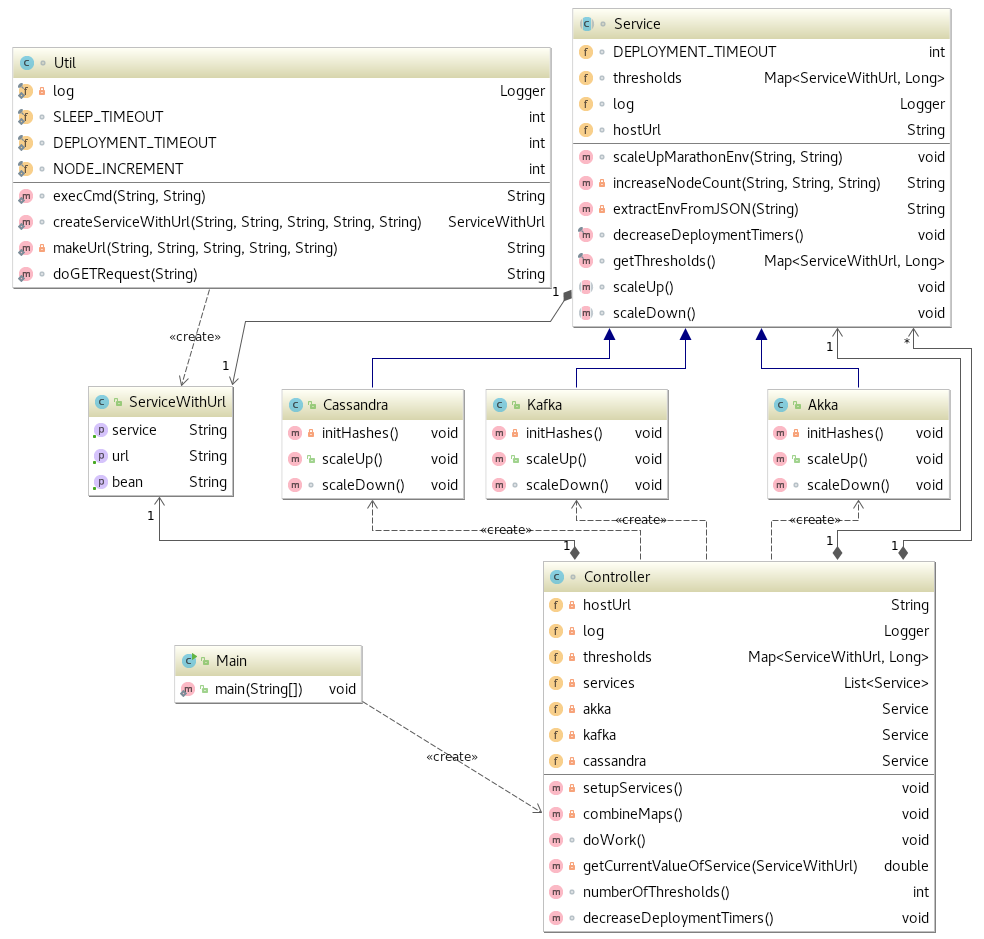
\includegraphics[keepaspectratio=true,scale=0.45]{img/smack_controller_uml}
    \caption{SMACK Controller}
    \label{fig:smack_controller_uml}
\end{figure}



\section{Framework Management Tools and Predefined Blueprints}
The launching and facilitating of a big data stack can get complex and thus automated deployments can help to minimize setup pitfalls.
This section introduces a management tool to quickly deploy the SMACK stack in the cloud, as well as configuration blueprints.

\subsection{Launching Tool}
Launching and setting up a Big Data stack with a cluster abstraction in the cloud is for sure not a trivial task.
To dramatically reduce the manual effort, in the course of this thesis, some tools are used which are described in this section.
AWS provides a Cloud Formation (CF) service, which enables the user to create templates of cloud deployments.
Any kind of AWS resource can be instantiated, configured, mounted or terminated in the template.
It helps system administrators and developers to easily setup a desired running configuration with a few clicks.\\
The CF templates are simple JSON files, which can be created by copying a template from AWS or using the AWS CF template online editor.
A benefit of using CF is that it is also possible to update running stacks, like adding additional nodes etc.
This requires no special update flag, but only the upload of the existing template with the updated values and AWS CF automatically recognizes what has changed and accordingly updates the instances.\\

In this thesis DC/OS (DataCenter OperatingSystem) \cite{dcos}, is used to run the SMACK stack in the cloud.
It is basically an open source, distributed operating system which uses Mesos as its system kernel.
The advantage to use DC/OS is that it leverages the setup of Mesos on multiple nodes and joining them together to one cluster.
In addition there are application packages available for most big data frameworks.
This means, once it is set up, installing Apache Spark is just as much as selecting the package and clicking on install.
DC/OS takes care of launching everything, opening ports, registering nodes etc.\\

Fortunately there is a predefined AWS Cloud Formation template available to launch DC/OS in the cloud offered by DC/OS itself.
Zuehlke Engineering AG provides a repository \cite{shmack} with some handy tools to even more automate the launch of the stack.
The repository offers a configuration file with which all necessary AWS launch parameters can be set and additional bash scripts to gather information once the stack is up and running.\\
As part of this thesis, the used version of DC/OS is updated and several additional helper scripts are provided.
This includes a command to deploy all SMACK components and further install the desired application itself into the stack.
To help new users get into deeper understanding and avoid starting problems, the respective documentation has been updated.


\subsection{Blueprints}
As part of the contribution, reference deployment architecture and configuration, or simply deployment blueprints are produced.
This information is the result of experimenting with resource distribution and scaling up and down services.
The blueprints are given for two kinds of applications running in the SMACK stack, I/O and computational bound.
It is therefore as good entry point when setting up the stack initially, without having to bother with experimenting on how to distribute the resources ideally.\\
During the experiments with the applications described in Section~\ref{sec:iot_application} and Section~\ref{sec:computation_application}, the resource workload is evaluated and based on that results, the deployment architecture and configurations are deduced.
It can be especially useful to have these configurations, if one does not have a lot of experience with the SMACK stack, but still wants to get the most out of the provided resources.\\

In Table~\ref{tab:blueprint-io} the recommended distribution of CPU and RAM for the respective frameworks is listed for a typical I/O intense application, assuming that Akka serves as data ingestion point.\\
Obviously Mesos is not part of the table, as it is the resource manager.
Akka has to handle a lot of requests, which justifies that it gets the most resources.
Depending on how much logic the ingestion application has to perform, CPU is slightly more important than just a lot a memory.\\
Cassandra is in the end of the data pipeline and uses mainly disk storage.
Still this has shown to be sufficient for writing a lot of data, especially because of the master-less and redundant design of Cassandra.\\
Kafka has to handle lots of pre-processed data and - depending on how many consumers there are - needs to stream data to many nodes.
This requires computational power as well as enough memory to be performant and not being the bottleneck.\\
In this context, Spark as the computation engine of the data pipeline, does not have to do a lot of heavy number crunching, but still relies - per design - on enough memory to perform well.\\


Table~\ref{tab:blueprint-computational} gives the recommendation of how to initially launch a computational bound application within the SMACK stack.\\
In this scenario the data ingestion with Akka does not require many resources as there will not be many connections to handle.
Also Kafka will not be under a lot of stress as a consequence.\\
The most work will be done by Spark when performing the heavy computations.
In this case, enough resources are a good idea so that Spark can spawn enough executors and allow those to perform in-memory computations.\\
The recommendation is also to give Cassandra slightly more resources than in the previous setup, as Spark will have to communicate a lot with the database.

\begin{table}[]
\begin{tabular}{lrrr}
\toprule
                   & \textbf{CPU} & \textbf{RAM} \\ \midrule
\textbf{Akka}      & 35\%         & 30\%  \\
\textbf{Cassandra} & 15\%         & 10\%  \\
\textbf{Kafka}     & 35\%         & 35\%  \\
\textbf{Spark}     & 15\%         & 25\%  \\
\bottomrule
\end{tabular}
\centering
\caption{Deployment Blueprint: I/O Bound Application}
\label{tab:blueprint-io}
\end{table}


\begin{table}[]
\begin{tabular}{lrrr}
\toprule
                   & \textbf{CPU} & \textbf{RAM} \\ \midrule
\textbf{Akka}      & 10\%         & 10\%  \\
\textbf{Cassandra} & 25\%         & 25\%  \\
\textbf{Kafka}     & 15\%         & 15\%  \\
\textbf{Spark}     & 50\%         & 50\%  \\
\bottomrule
\end{tabular}
\centering
\caption{Deployment Blueprint: Computational Bound Application}
\label{tab:blueprint-computational}
\end{table}


\begin{table}[]
\begin{tabular}{@{}lp{7.5cm}l@{}}
\toprule
MBean & Description & Attributes \\ \midrule
UnderReplicatedPartitions     &  This is an indicator of availability and the value should exceed zero only for a short time.
                                 Longer periods of under replication are an indicator of potential problems with Kafka's high-availability.
                                 & Value \\
ActiveControllerCount         &  Equals the number of active controller within the Kafka cluster.
                                 In each cluster there has to be exactly one controller.
                                 This is an urgent indicator for errors if the value zero.
                                 & Value \\
OfflinePartitionsCount        &  In case a partition loses its leader, it goes offline and becomes inaccessible by producers and consumers.
                                 This is because all operations have to be performed by the leader.
                                 Any value above zero is alarming.
                                 & Value \\
UncleanLeaderElectionsPerSec  &  The metric is a good indicator for data loss, as every topic must have a leader.
                                 In case a leader gets offline and Kafka is not able to elect a new one, an out-of-sync replica will be elected, even if it means that some messages are lost forever.
                                 Any value above zero should be considered as potential error.
                                 & OneMinuteRate \\
TotalTimeMs Produce           &  Indicates the total time it takes Kafka to serve a request.
                                 In this case it is the time from the producer's request until the data is sent.
                                 The metric comprises the time in the queue, local processing time of the leader, waiting time of the followers and the time to send respond.
                                 Big fluctuations and suspiciously long waiting times are indicators for performance problems.
                                 & Count, Mean \\
TotalTimeMs FetchConsumer     &  Same as above, but the time from the consumer's request until the data is received.  & Count, Mean \\
TotalTimeMs FetchFollower     &  Same as above, but the time from the broker's follower request until the data is received
                                 & Count, Mean \\
BytesInPerSec                 &  Gives information of how many bytes per second are received.
                                 Can be an indicator if an upper bound of the system is known by experimenting.
                                 & OneMinuteRate \\
BytesOutPerSec                &  Same as above, but the bytes send per second.  & OneMinuteRate \\
\bottomrule
\end{tabular}
\centering
\caption{Relevant Kafka JMX Metrics}
\label{tab:jmx_kafka}
\end{table}


\begin{table}[]
    \begin{tabular}{@{}p{3.2cm}p{2.7cm}p{6.7cm}p{2.2cm}@{}}
\toprule
MBean                                                & Scope             & Description & Attributes \\ \midrule
\textbf{ClientRequest}: Latency, TotalLatency                & Read, Write       &
                                                             Describes the latency of a client request.
                                                             The total value is accumulated in milliseconds while the latency count provides the number of events.
                                                             & OneMinuteRate, Count \\

\textbf{Cache}: Hits, Requests                               & KeyCache          &
                                                             The KeyCache hit rate indicates the percentage of how many of the read requests keys were found in the cache on disk.
                                                             This can be an indicator for performance loss if there are very little cache hits.
                                                             & Count \\
\textbf{Storage}: Load, Exceptions                           & n.a.              &
                                                             The load tells how many bytes per node are used by Cassandra.
                                                             With the exceptions count it is possible to determine how many errors - fatal and non-fatal - occurred on a node.
                                                             If this value is increasing, something goes wrong in the cluster.
                                                             & Count \\
\textbf{Compaction}: CompletedTasks, PendingTasks            & n.a.              &
                                                             Reflects the number of successful compaction tasks, respectively the ones in the waiting queue.
                                                             A lot of pending tasks is an indicator for potential overload on the cluster, as it is not enough time to compact the data.
                                                             & Value \\
\textbf{GarbageCollector}: ParNew, ConcurrentMarkSweep       & n.a.              &
                                                             The ParNew is the young-generation Java garbage collector in the JVM.
                                                             Everytime it frees up unused memory all application threads get paused and thus it directly affects the performance of Cassandra.
                                                             While ConcurrentMarkSweep does not block all threads it handles the old-generation part of the JVM heap.
                                                             An increasing value of the garbage collector execution is an indicator for too little RAM in the cluster.
                                                             & CollectionCount, CollectionTime \\
\textbf{ThreadPools}: PendingTask, CurrentlyBlockedTasks     & MutationStage, ReadRepairStage, ReadStage, RequestResponseStage        &
                                                             This MBean gives information about pending and blocked tasks in the thread pools.
                                                             In the RequestResponseStage all callbacks to responses to a request are executed with the original request.
                                                             The ReadStage comprises the execution of a local read including cache deserialization.
                                                             In the MutationStage inserts, updates, schema merges and log replays are performed.
                                                             The ReadRepairStage executes read repairs if necessary.
                                                             The increase of the count in those metrics could mean that there is a disk issue, overload or some performance problem with Cassandra.
                                                             & Count \\
\bottomrule
\end{tabular}
\centering
\caption{Relevant Cassandra JMX Metrics}
\label{tab:jmx_cassandra}
\end{table}


\begin{table}[]
\begin{tabular}{@{}lp{8cm}l@{}}
\toprule
MBean & Description & Attributes \\ \midrule
ProcessingTime                & The absolut time to process a received message.
                                If the value exceeds a certain threshold it is very likely that Akka is running out of resources.
                              & Max, Sum \\
KBytes per Second             & As the name indicates, it referrs to the number of KB input per second.
                                Knowing the underlying system this can be a warning indicator if there is too much data to handle for Akka.
                              & Avg \\
Messages per Second           & Same as above but messages per second.
                                The value does not necessarily correlate with the KB/s, as messages can vary dramatically in size.
                              & Avg \\
TimeInMailbox                 & Equals the absolute time a message is kept in an actors mailbox.
                                This metric is a very good indicator for an overload of Akka, as the value usually fluctuates only very little, an increase of it means that Akka is running out of resources.
                              & Sum \\
MailboxSize                   & This metric corresponds to the absolute mailbox size of an actor.
                                Same as time in mailbox, there is no significant fluctuation during regular load on the system.
                                As the value increases, Akka is going to run out of resources very soon.
                              & Sum \\
Errors                        & A value above zero means, that there happend some major errors during the runtime of the application.
                              & Count \\
\bottomrule
\end{tabular}
\centering
\caption{Relevant Akka JMX Metrics}
\label{tab:jmx_akka}
\end{table}



\begin{table}[]
\begin{tabular}{@{}lp{8cm}l@{}}
\toprule
MBean & Description & Attributes \\ \midrule
DAGScheduler.messageProcessingTime                        & Indicates how long it takes Spark to process one message at a time. If this value is increasing it is a very good indicator that the application needs more resources.
                              & OneMinuteRate \\
DAGScheduler.stage.runningStages                        & This metric represents the amount of stages running in parallel. This value should not be zero as it would mean that no processing is done.
                              & Value \\
DAGScheduler.stage.waitingStages                        & In case this value increases steadily, Spark is not able to handle new requests or tasks quick enough. It is an indicator for insufficient resources.
                              & Value \\
BlockManager.memory.memUsed\_MB                        & It is interesting to keep an eye on the used memory to see whether Spark is already close to the limit of what is provided or not.
                              & Value \\
streaming.totalProcessedRecords                        & The amount of totally processed records should steadily increase. A stagnation is an indicator that Spark cannot perform its tasks anymore.
                              & Value \\
\bottomrule
\end{tabular}
\centering
\caption{Relevant Spark JMX Metrics}
\label{tab:jmx_spark}
\end{table}



%%%%%%%% CHAPTER %%%%%%%%%
\chapter{Evaluation}
\label{ch:evaluation}
This chapter gives an overview of the results and how the benchmark is set up.
The used tools and relevant metrics are introduced for the respective technologies.
Further the evaluation criteria is given and the summary of the results is discussed.

\section{Setup and Methodology}
\label{sec:evaluation_setup}
In order to evaluate the framework's performance, a use-case based approach with two real-world applications is chosen.
In the course of this thesis following two applications are used for the experiments:\\
The first application is designed to mainly deal with I/O operations, based on IoT data, is described in section \ref{sec:iot_application}.
To get the SMACK stack close to its limit the load generator and stress test tool introduced in section \ref{sec:load_generator} are used.\\
The second application used to evaluate the auto-scaling framework is introduced in section \ref{sec:computation_application}.
As the scenario here is fundamentally different, it is a good indicator whether the framework is able to correctly monitor and scale the stack or not.
Most of the computation power is needed in Apache Spark, which the framework should detect and assign the most resources to this service.\\


\subsection{Load Generator and Stress Test}
\label{sec:load_generator}
To be able to test the application described in Section~\ref{sec:iot_application} a load generator was designed.
The tool has two modes - either pre-recorded real life IoT sensor data, or random data, can be send to the cluster.\\
In principle the tool just sends lots of HTTP requests to the server, while the JSON data is not interpreted and only treated as plain string.
In the random mode, only the timestamp of the entries is randomized, as it is enough to cause unique entries in the Cassandra database.\\

The mode with real data requires the data to be provided in a specific format.
In the source code there is a tool for formatting JSON files into the proper format to be used further.
As one HTTP request contains a whole sensor data JSON entry of a device, it is of favor, to concatenate the entries into a single line.
This reduces the CPU load, as the parsing can be omitted and one line equals one request.
With the help of the provided tool, text files with multiple JSON entries can be joined together to one larger text file containing single-line entries.
The advantage of using a few large files over multiple smaller files is that the disk time can be reduced dramatically during reading, which causes higher throughput.\\
In addition the milliseconds of the timestamp of each entry is randomize to avoid duplicates in the database.
This has to be done at runtime and cannot be pre computed in advance.\\

The contribution of this thesis to the tool is the optimization of the data format, as well as integrating randomization to achieve unique database entries even when the tools runs in parallel with the same input data.\\

To be able to orchestrate multiple clients at once, the load generator is deployed into a Docker image.
AWS provides a service called \textit{Elastic Cloud Computing Container Service (ECS)}.
It allows the user to easily deploy, manage and scale Docker containers in a managed cluster.\\
There are a few advantages of using this service: It is as easy as clicking on "scale" to instantiate more containers and distribute them equally across the cluster.
Amazon allows the user to configure how the containers are distributed, for example place each container on a different node to provide equal stress among the cluster, or to pack everything on one node until its working capacity is full.
In addition many other AWS services are integrated, like Elastic Load Balancing, etc.
An important feature is the command line API, which helps to automatically launch and stop instances in the cluster.\\

In Figure~\ref{fig:aws_ecs} the service is illustrated and shows the individual components.
The unit of execution is always a Docker image, which can be pulled from any available container registry.
It is possible to use mainstream platforms like Docker Hub, host it at Amazon or provide a self-hosted solution.\\
Next, ECS requires the user to create a so called task definition, which is basically a JSON file which contains parameters like the container name, open ports, CPU and memory resources, mappings, etc.
There is also a web interface to easily create a task without having to write JSON.
Now it is possible to launch and stop tasks with AWS ECS doing all the work of distributing and running the container images with the correct parameters across the cluster.
Further a service can be created which defines different scheduling options and can be used to maintain a desired number of container instances or tasks executing simultaneously.\\

All the containers run inside a Virtual Private Cloud (VPC), which helps to easily integrate the cluster in existing solutions.
Amazon also provides the option to create a dedicated VPC for the ECS cluster without any configuration effort.
The cluster itself is a logical grouping of AWS Elastic Cloud Computing (EC2) instances, which can run in different Availability Zones (AZ).
This allows the user to logically distribute clusters and reduce network latency.
To be able to execute tasks and monitor the EC2 instances used for the ECS service, a container agent is running on each node and provides the AWS ECS controller with information and allows autonomous interaction.\\

To be able to run the load generator in the cloud by using AWS ECS, the creation of a Docker image, containing all necessary sensor data, was performed as part of this thesis.
Additionally the required task definition was created and a simple bash script to launch an arbitrary number of container instances in the cluster.


\begin{figure}[!htbp]
  \centering
  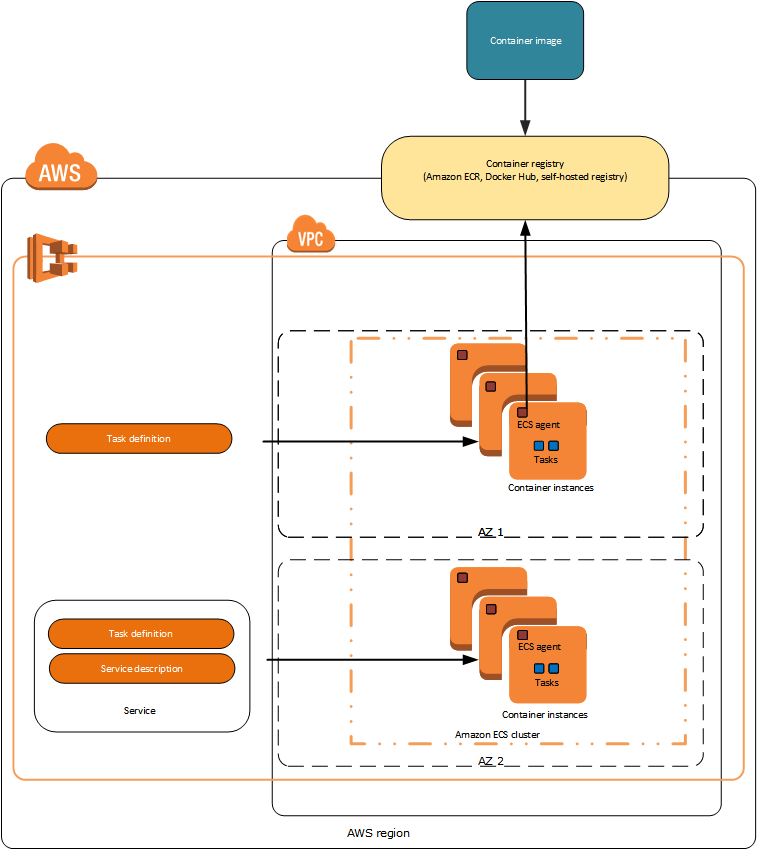
\includegraphics[keepaspectratio=true,scale=0.75]{img/aws_ecs}
    \caption{Overview of Amazon WebServices Elastic Cloud Computing Container Service \cite{aws}}
  \label{fig:aws_ecs}
\end{figure}


\subsection{Sensor Data Overview}
\label{sec:sensor-data}
The data used for the IoT application comes from sensors in elevators which were used during the HackZurich.
Mobile phones were placed inside the elevators and used to gather various information about like acceleration, noise, light, etc.\\
In this section the available data is listed and explained in roughly.

\begin{itemize}
    \item Accelerometer\\
          "It is a measurement of acceleration along the three spatial axes at a moment of time" \cite{sensor-data}.
    \item Gyrometer\\
          This gives information about the device rotation rate.
    \item Magnetometer\\
          Gives information about the measured magnetic field surrounding the device. The unit is microteslas.
    \item DeviceMotion\\
          "The data represents measurements of the attitude, rotation rate, and acceleration of a device" \cite{sensor-data}.
    \item Barometer\\
          Indicates the relative changes of altitude.
    \item BatteryLevel\\
          Gives information about the remaining battery of the device.
    \item Microphone\\
          Represents the recorded noise in dB.
    \item Light\\
          The ambient sensor is used to determine how bright the light is.
    \item Beacon\\
          Any beacon recorded during the monitoring is represented by this class.
\end{itemize}

\begin{code}
\begin{minted}[frame=single,framesep=10pt,fontsize=\scriptsize,linenos]{json}
[
   {
      "z":-1.003677368164062,
      "x":-0.0066986083984375,
      "y":-0.036865234375,
      "date":"2016-09-05T14:49:18.413+02:00",
      "type":"Accelerometer"
   },
   {
      "z":-0.003133475338587232,
      "x":-0.06178427202540229,
      "y":0.07116925170684153,
      "date":"2016-09-03T08:40:17.552+02:00",
      "type":"Gyro"
   },
   {
      "z":-645.7014770507812,
      "x":-19.19688415527344,
      "y":140.535400390625,
      "date":"2016-09-05T14:50:23.371+02:00",
      "type":"Magnetometer"
   },
   {
      "attitude":{
         "quaternion":{
            "x":0.0180332360021854,
            "w":0.9998316704300516,
            "y":-0.003365478874680562,
            "z":-0.0003267357948271106
         },
         "rotationMatrix":{
            "m13":0.006718040909618139,
            "m12":-0.0007747425115667284,
            "m33":0.9993269443511963,
            "m32":-0.0360582023859024,
            "m31":-0.006741608958691359,
            "m21":0.0005319805932231247,
            "m11":0.9999771118164062,
            "m22":0.9993494153022766,
            "m23":0.03606259822845459
         },
         "pitch":-0.006722463864462229,
         "yaw":-0.000722464864462227,
         "roll":-0.001732463864562228
      },
      "date":"2016-09-05T14:49:26.286+02:00",
      "type":"DeviceMotion"
   },
   {
      "relativeAltitude":0,
      "pressure":95.66769409179688,
      "date":"2016-09-05T14:50:26.300+02:00",
      "type":"Barometer"
   },
   {
      "type":"Battery",
      "date":"2016-09-05T14:49:18.413+02:00",
      "batteryLevel":"1.0",
      "batteryState":"Full"
   },
   {
      "peakPower":-24.93737,
      "averagePower":-31.9056,
      "date":"2016-09-05T14:50:23.736+02:00",
      "type":"Microphone"
   },
   {
      "type":"Light",
      "date":"2016-09-05T14:49:18.413+02:00",
      "brightnes":"0.3414323"
   },
   {
      "beacons":[
         {
            "accuracy":4.084238652674522,
            "id":"F7826DA6-4FA2-4E98-8024-BC5B71E0893E",
            "major":59314,
            "rssi":-88,
            "minor":13391
         },
         {
            "accuracy":4.641588833612778,
            "id":"F7826DA6-4FA2-4E98-8024-BC5B71E0893E",
            "major":60085,
            "rssi":-89,
            "minor":55763
         }
      ],
      "date":"2016-09-13T10:04:04.034+02:00",
      "type":"Beacon"
   }
]
\end{minted}
\captionof{listing}{Sensor Data Content Example \cite{sensor-data}}
\end{code}



More detailed information can be found in the hackzurich-sensordata-ios repository \cite{sensor-data-repo}.


\subsection{Experiment Setup}
The goal of the experiment is to find out how well the scaling tool impacts the performance of the SMACK stack.
This section describes the experiment setup and which steps are taken to collect evaluation data.

\subsubsection{IoT Application}
In case of the IoT-application the following setup is chosen, which is also reflected by the architecture illustrated in Figure~\ref{fig:overall_view}:

\begin{enumerate}
\item Launch the REST Monitor.
\item Launch the DC/OS cluster.
\item Deploy the SMACK stack.
\item Launch the JMX Extraction tool.
\item Deploy the IoT application.
\item Instantiate the ECS Load Generator. \label{enum:load_generator_start}
\item Slowly increase the load by adding Docker container instances to ECS.\\
      Slowly means five new containers each minute until 50 instances are up to give the application and the SMACK stack time for warm-up.
      Then two containers per minute are launched until 70 containers are running.
      After that, one container per minute is added.
\item Evaluate the extracted metrics to see how much data the single services can handle until the stack crashes.\\
      Whether the stack is still healthy or not is determined by looking at the DC/OS health status of each service.
      In addition the Akka application provides a web interface with simple statistics which will be unavailable once the service crashes.
\item Stop the ECS Load Generator. \label{enum:load_generator_stop}
\item Restart / redeploy unhealthy services.
\item Launch the Scaling Tool.
\item Perform steps \ref{enum:load_generator_start} to \ref{enum:load_generator_stop}.
\end{enumerate}

There are two runs which are almost identical.\\
In the first run, the stack is unsupervised and no resource re-distribution is performed.
This gives a baseline of how well the stack and the application perform in a default setup.
After the stack crashed all extracted metrics are stored in the REST Monitor which can be then used to determine 1) when the stack or one component crashed exactly and 2) how much data could be handled (total MB/s), as well as other metrics.
Additionally the information about the performance of each service is stored and can be evaluated.\\
In the second run the Scaling tool is launched, analyzing the stack and - if necessary - scaling services up or down.
Again, after the stack crashes under the heavy input of the load generator, the metrics stored in the REST Monitor are analyzed.\\

As there is now statistical data available of both runs, the conclusion of whether the tool worked as expected or not can be made.
It is expected that the ingestion part of the SMACK stack, which is Akka and Kafka, will crash first in this scenario, as the application is mainly IO-bound.\\

The configuration of Kafka, Cassandra and is set to the defaults used by DC/OS, while Akka is deployed within the custom application, which therefore needs a custom configuration.
This is shown in Source~Code~\ref{code:akka_iot_config}, which serves as input for the Marathon framework to deploy the application.

\begin{code}
\begin{minted}[frame=single,framesep=10pt,fontsize=\scriptsize,linenos]{json}
{
  "id": "sensor-ingestion",
  "instances": 1,
  "cpus":1,
  "mem":1048,
  "disk": 100,
  "container":{
    "docker":{
      "forcePullImage":true,
      "image":"bwedenik/sensor-ingestion",
      "network":"HOST",
      "privileged": false
    },
    "type":"DOCKER"
  },
  "labels":{
    "HAPROXY_GROUP":"external",
    "HAPROXY_0_PORT": "8083"
  },
  "portDefinitions": [
    {
      "port": 10099,
      "protocol": "tcp",
      "labels": {}
    },
    {
      "port": 10100,
      "protocol": "tcp",
      "labels": {}
    }
  ],
  "healthChecks": [
    {
      "protocol": "TCP",
      "path": "/hello",
      "portIndex": 0,
      "gracePeriodSeconds": 300,
      "intervalSeconds": 60,
      "timeoutSeconds": 15,
      "maxConsecutiveFailures": 3,
      "ignoreHttp1xx": false
    }
  ]
}
\end{minted}
\captionof{listing}{Marathon Configuration for Akka Sensor Ingestion Application}
\label{code:akka_iot_config}
\end{code}

The Spark driver for \textit{KafkaToCassandra}, which is the number crunching job to parse the incoming data and write it into the database, is configured with the following parameters:\\
\verb|spark.cores.max=2 --driver-memory 8G|\\
\verb|spark.driver.cores=2 spark.executor.cores=2 --executor-memory 4G|\\

\begin{minipage}{\linewidth}
\begin{code}
\begin{minted}[frame=single,framesep=10pt,fontsize=\scriptsize,linenos]{bash}
spark.executor.extraJavaOptions=-Dcom.sun.management.jmxremote=true \
 -Dcom.sun.management.jmxremote.port=8092 -Dcom.sun.management.jmxremote.ssl=false \
 -Dcom.sun.management.jmxremote.authenticate=false
spark.driver.extraJavaOptions=-Dcom.sun.management.jmxremote=true \
 -Dcom.sun.management.jmxremote.port=8092 -Dcom.sun.management.jmxremote.ssl=false \
 -Dcom.sun.management.jmxremote.authenticate=false
\end{minted}
\captionof{listing}{Spark JMX Deployment Configuration}
\label{code:spark_jmx_config}
\end{code}
\end{minipage}

Further, to be able to extract JMX values from Spark, the configuration shown in Source~Code~\ref{code:spark_jmx_config} is required when deploying the driver.


\subsubsection{Acceleration Prediction Application}
The scenario of running this application in the SMACK stack is very similar to the previous one:

\begin{enumerate}
\item Launch the REST Monitor.
\item Launch the DC/OS cluster.
\item Deploy the SMACK stack.
\item Launch the JMX Extraction tool.
\item Instantiate the IoT application.
\item Instantiate the ECS Load Generator (only a few instances to not overload the system).
\item Wait for the database to be filled sufficiently.
\item Deploy the prediction application.
\item Let the data pipeline and the application work until enough predictions are provided. \label{enum:prediction_work}
\item Evaluate the extracted metrics to see how well the application performs. \label{enum:prediction_evalutation}
\item Restart / redeploy unhealthy services.
\item Launch the Scaling Tool.
\item Execute step \ref{enum:prediction_work} and \ref{enum:prediction_evalutation}.
\end{enumerate}

As described before, there are two runs required, one with and one without the Scaling Tool.
The difference between both runs is then analyzed and evaluated to conclude the performance of the Scaling Tool.
It is important to mention again, that the IoT application is launched in this scenario with a dramatically reduced load from the ECS Load Generator.
There is just the need of IoT data in the database, but not a heavy ingestion load.

The Prediction Data Analytics application itself is configured like this:\\
\verb|spark.cores.max=1 --driver-memory 2G|\\
\verb|spark.driver.cores=1 spark.executor.cores=1 --executor-memory 1G|\\
Also for this setup, the configuration from Source~Code~\ref{code:spark_jmx_config} is required when deploying the Spark driver.


\subsubsection{Evaluation Criteria}
\label{sec:evaluation_criteria}
As not only RAM and CPU, but more specific characteristics like Akka's mailbox size are considered, relevant metrics are presented with respect to the evaluated application.

\subsubsection{IoT Data Storage Application}
In this application metrics concerning the data throughput are interesting.
To give a more complete of the whole stack some metrics are included which are not directly related to throughput or latency.
The relevant metrics are illustrated in Table~\ref{tab:metrics_iot}.\\

\begin{table}[]
\begin{tabular}{lp{5cm}p{8cm}}
\toprule
Technology & Metric & Description \\ \midrule
Akka & KB per Second & \\
     & Messages per Second & \\
     & Processing Time & How long does it take to process one message.\\
     & Time in Mailbox & How long does one message have to wait in the mailbox until it is processed.\\
     & Mailbox Size & Number of total messages in the mailbox.\\
Kafka & Bytes Out per Second & \\
      & Bytes In per Second & \\
      & Total Time Produce & Total time it takes Kafka to serve a request.\\
      & Total Time FetchFollow & Total time from the consumer's request until the data is received.\\
      & Total Time FetchConsumer & Total time from the broker's follower request until the data is received.\\
      & Offline Partitions & In case a partition loses its leader, it goes offline and becomes inaccessible by producers and consumers.\\
      & Under Replicated Partitions & Indicates how many partitions are currently not replicated fully.\\
Cassandra & Read Latency & \\
          & Write Latency & \\
          & Load & \\
Spark & Message Processing Time & \\
      & Memory Used & \\
      & Total Processed Records & \\
\bottomrule
\end{tabular}
\centering
\caption{Relevant IoT Data Storage Application Metrics}
\label{tab:metrics_iot}
\end{table}

\subsubsection{Acceleration Prediction Application}
\label{sec:evaluation_prediction_application}
As the setup of this application is only computational bound, it is not important to consider the throughput of the Akka data ingestion and how many bytes were managed by Kafka.
The scenario focuses on the performance of the acceleration prediction, which happens in the Spark job.
Therefore only Spark metrics are considered.\\
In the course of this thesis only the build-in Spark metrics are considered, which reduces the interesting ones illustrated in Table~\ref{tab:metrics_prediction}.\\


\begin{table}[]
\begin{tabular}{lp{5cm}p{8cm}}
\toprule
Technology & Metric & Description \\ \midrule
Spark & Message Processing Time & Indicates how long it takes Spark to handle and process a single message.\\
      & Complete Tasks & With this metric one can tell how many tasks were finished by Spark.\\
\bottomrule
\end{tabular}
\centering
\caption{Relevant Acceleration Prediction Application Metrics}
\label{tab:metrics_prediction}
\end{table}



\section{Results}
This section comprises the results of the executed benchmarks.
The generated plots of the described metrics are described and compared with each other.\\

To be able to better compare the values, two more variations of diagrams are added:
\begin{itemize}
    \item \textbf{Average}:\\
        The average values of all nodes, implemented With a shifting time window.
        This can be used for metrics like time-in-mailbox, mailbox-size, and so on.
        The caption is in form of \verb|Attribute_avg|
    \item \textbf{Sum}:\\
        Summed up values, also implemented with a shifting time window.
        This can be used for metrics like kbytes-per-second, messages-per-second, etc.
        The caption is in form of \verb|Attribute (sum)|
\end{itemize}


% Command to insert a plot
\newcommand{\plot}[3]{ \plotsize{#1}{#2}{#3}{0.30} }
\newcommand{\plotsize}[4]{
\begin{figure}[h]
  \centering
  \includegraphics[keepaspectratio=true,scale=#4]{img/results/#1}
    \caption{#3}
  \label{fig:#2}
\end{figure}
}

\subsection{IoT Data Storage Application}
\subsubsection{Akka}
In Figure~\ref{fig:without_akka_kbytes_per_second} one can see how many kilo bytes are handled by the Akka ingestion application without the help of the Scaling Tool.
First there is no input, as the stack is still launching and the load generator was not started.
After that, a steadily increasing load gets up to about 24 MB/s (= 192 MBit/s), but does not exceed the value.
Apparently then the application was under too heavy load and the load generator was stopped.
After a recovery phase, the load was again increased steadily, this time reaching up to 34 MB/s (= 272 MBit/s).\\
Figure~\ref{fig:with_akka_kbytes_per_second_separate} shows the same metric (each host is illustrated separately), but with the interacting scaling tool.
Additionally Figure~\ref{fig:with_akka_kbytes_per_second_sum} is showing the summed up ingested kilo bytes and displays only one curve for a better comparability.
One can observe, that that after a certain load, new instances were added by the Scaling Tool.
Further, there is one instance which was killed by Mesos and restarted later on.\\
The increase of the load is similar to the previous experiment: First there is so much load added that the system gets under too much stress and after a recovery phase, the load is steadily increased again.
In this scenario the peak is at about 59 MB/s (= 472 MBit/s).\\

Figure~\ref{fig:without_akka_messages_per_second}, \ref{fig:with_akka_messages_per_second_separate} and \ref{fig:with_akka_messages_per_second_sum} show a very similar behavior, as they represent the received messages per second.\\
As one can see, there is this a sudden drop of messages-per-second in Figure~\ref{fig:with_akka_messages_per_second_sum}.
This is a result of the sliding time window, as for this timestamp there is apparently just the information of one node available, which is then of course a lower value than when adding multiple ones.
A clear observation which can be made, is that the run with the Scaling Tool performs better in terms of throughput.\\

Concerning the message processing time, Figure~\ref{fig:without_akka_processing_time} shows a similar development as the messages per second and kilo bytes per second.
The time increases steadily, reaches the plateau, drops to zero and then increases steadily after the recovery phase.
An increase of the processing time, means directly that the system gets under more stress and the respons time gets slower.\\
Figure~\ref{fig:with_akka_processing_time_separate} illustrates the same metric but with enabled Scaling Tool, as well as Figure~\ref{fig:with_akka_processing_time_avg}, but with an averaged values over all hosts.
As one can see, the message processing time develops a bit smoother than the previous metrics.
The increase is not as steep and in the runs with the Scaling Tool, the three running instances provide an adequate processing time even under heavy load.
This behavior is desired and the response time is distributed equally between the nodes, according to the plot.\\

Related to the processing time, there is the time in mailbox metric which is illustrated in Figure~\ref{fig:without_akka_time_in_mailbox} for the run without the Scaling Tool.
Here the dramatically high peak indicates, that the system cannot process the messages in time anymore.
The sudden increase gives a hint, that at the given time, the Akka application started to become unresponsive.
Comparing this with Figure~\ref{fig:with_akka_time_in_mailbox_separate} and Figure~\ref{fig:with_akka_time_in_mailbox_sum}, which are the plots of the Scaling Tool run, one can observe, that although there is a high peak right at the beginning of the run, the system was able to recover immediately and the freshly added instances had a significantly lower value than the existing one.
This could be because the mailbox of the existing instance is already filled with messages, while the new instances obviously start with an empty mailbox.
Similar as in the processing time plots, the load is evenly balanced between the instances in the second half of the run, as the load is increased.\\
The mailbox size itself is displayed in Figure~\ref{fig:without_akka_mailbox_size}, where the experiment is performed without the Scaling Tool and in Figure~\ref{fig:with_akka_mailbox_size_separate} and Figure~\ref{fig:with_akka_mailbox_size_sum} with the enabled tool.
As expected, the mailbox size correlates to the message processing time and the time in mailbox.



% Akka KBytes per second
\plot{iot_before/akka_kbytes_per_second}{without_akka_kbytes_per_second}{Akka, Without Scaling Tool, KBytes per Second}
\plot{iot_after/akka_kbytes_per_second_separate}{with_akka_kbytes_per_second_separate}{Akka, With Scaling Tool, KBytes per Second, Separated by Host}
\plot{iot_after/akka_kbytes_per_second_sum}{with_akka_kbytes_per_second_sum}{Akka, With Scaling Tool, KBytes per Second, Summed up}

% Akka messages per second
\plot{iot_before/akka_messages_per_second}{without_akka_messages_per_second}{Akka, Without Scaling Tool, Messages per Second}
\plot{iot_after/akka_messages_per_second_separate}{with_akka_messages_per_second_separate}{Akka, With Scaling Tool, Messages per Second, Separated by Host}
\plot{iot_after/akka_messages_per_second_sum}{with_akka_messages_per_second_sum}{Akka, With Scaling Tool, Messages per Second, Summed up}

% Akka processing time
\plot{iot_before/akka_processing_time}{without_akka_processing_time}{Akka, Without Scaling Tool, Processing Time}
\plot{iot_after/akka_processing_time_separate}{with_akka_processing_time_separate}{Akka, With Scaling Tool, Processing Time, Separated by Host}
\plot{iot_after/akka_processing_time_avg}{with_akka_processing_time_avg}{Akka, With Scaling Tool, Processing Time, Averaged over Hosts}

% Akka time in mailbox
\plot{iot_before/akka_time_in_mailbox}{without_akka_time_in_mailbox}{Akka, Without Scaling Tool, Time in Mailbox}
\plot{iot_after/akka_time_in_mailbox_separate}{with_akka_time_in_mailbox_separate}{Akka, With Scaling Tool, Time in Mailbox, Separated by Host}
\plot{iot_after/akka_time_in_mailbox_sum}{with_akka_time_in_mailbox_sum}{Akka, With Scaling Tool, Time in Mailbox, Summed up}

% Akka mailbox size
\plot{iot_before/akka_mailbox_size}{without_akka_mailbox_size}{Akka, Without Scaling Tool, Mailbox Size}
\plot{iot_after/akka_mailbox_size_separate}{with_akka_mailbox_size_separate}{Akka, With Scaling Tool, Mailbox Size, Separated by Host}
\plot{iot_after/akka_mailbox_size_sum}{with_akka_mailbox_size_sum}{Akka, With Scaling Tool, Mailbox Size, Summed up}


\subsubsection{Kafka}
In the data pipeline, Kafka is the second element and gets its data directly from the Akka ingestion application, while the Spark job is polling from the topic.
The consumed data is measured in bytes per second, once illustrated as separate curve per host, once summed up to be better comparable.
Figure~\ref{fig:without_kafka_bytes_in_separate} and Figure~\ref{fig:without_kafka_bytes_in_sum} show the results of the run before the Scaling Tool is active,
while Figure~\ref{fig:with_kafka_bytes_in_separate} and Figure~\ref{fig:with_kafka_bytes_in_sum} illustrate the same metric with the tool being enabled.\\
The curves are similar to the ones in Figure~\ref{fig:without_akka_kbytes_per_second}, \ref{fig:with_akka_kbytes_per_second_separate} and \ref{fig:with_akka_kbytes_per_second_sum}, where the consumed bytes of Akka are shown.
The highest value of the uncontrolled run is about 33 MB/s, while the supervised one reaches up to 57 MB/s in total, which is expected, as Akka was already able to process more data.
An interesting observation is, that the load is not distributed equally between the Kafka brokers.
For example the peak of 29 MB/s one node \verb|10-0-3-37| is about 371\% higher than the one of \verb|10-0-0-6| with just 7.8 MB/s, illustrated in Figure~\ref{fig:with_kafka_bytes_in_separate}.
The phenomena of the sudden drops in the \textit{summed up} plots was already explained above but should be mentioned here again as it occurs in Figure~\ref{fig:with_kafka_bytes_in_sum} and a result of the sliding time window.\\
The "BytesOutPerSecond" curve develop very similar to the consumed bytes and can be seen in Figure~\ref{fig:without_kafka_bytes_out_separate}, \ref{fig:without_kafka_bytes_out_sum}, \ref{fig:with_kafka_bytes_out_separate} and \ref{fig:with_kafka_bytes_out_sum}.\\

To see whether Kafka got under too heavy stress, it is required to evaluate, whether there where any under replicated or even offline partitions.
In the run without the Scaling Tool the load was apparently not heavy enough to bring Kafka down, which is reflected in no under replicated partitions, Figure~\ref{fig:without_kafka_under_replicated_partitions}, and no offline partitions, which can be seen in Figure~\ref{fig:without_kafka_offline_partitions}.
During the experiment with enabled Scaling Tool, the load became too much for Kafka to handle it and partitions were lost.
Close to the peak of processed bytes, there were up to 53 under replicated partitions, Figure~\ref{fig:with_kafka_under_replicated_partitions}, and two partitions were offline, illustrated in Figure~\ref{fig:with_kafka_offline_partitions}.\\

Part of the collected metrics are the fetch consumer, fetch follower and produce time, which give an insight in how quick Kafka can interact with consumers and producers.
In Figure~\ref{fig:without_kafka_time_fetch_consumer_separate}, which reflects the total time in milliseconds of fetching a consumer, the run before enabling the Scaling Tool is shown.
When inspecting the plot, one can observe again that the load is not distributed equally between the nodes.
Further the maximum is at about 12000 ms on node \verb|10-0-0-6|, while the maximum in Figure~\ref{fig:with_kafka_time_fetch_consumer_separate} is about 10240 on the same node but with higher load, as the Scaling Tool already scaled up Akka and the load generator fired more requests.
Interestingly, there are less fluctuations, which could be because the Spark job polls less frequently due to the larger amounts of data.\\
Another maybe surprising outlier can be seen in Figure~\ref{fig:without_kafka_time_fetch_follower_separate} where the total time for fetching a follower increases dramatically as the data ingestion starts.
After about 12 minutes the service recovers and the time starts to decrease and stabilize.
This initial peak is not present in Figure~\ref{fig:with_kafka_time_fetch_follower_separate}, which represents the latter run, possibly because there is no initial phase and the brokers were already warmed up.\\
The same interesting behavior occurs when measuring the produce time, as illustrated in Figure~\ref{fig:without_kafka_time_produce_separate}, but not as dramatic as for the fetch follower time.
Similarly the produce time shows no outliers in the run with the Scaling Tool enabled, illustrated in Figure~\ref{fig:with_kafka_time_produce_separate}.


% Kafka bytes in
\plot{iot_before/kafka_bytes_in_separate}{without_kafka_bytes_in_separate}{Kafka, Without Scaling Tool, Bytes In, Separated by Host}
\plot{iot_after/kafka_bytes_in_separate}{with_kafka_bytes_in_separate}{Kafka, With Scaling Tool, Bytes In, Separated by Host}
\plot{iot_before/kafka_bytes_in_sum}{without_kafka_bytes_in_sum}{Kafka, Without Scaling Tool, Bytes In, Summed up}
\plot{iot_after/kafka_bytes_in_sum}{with_kafka_bytes_in_sum}{Kafka, With Scaling Tool, Bytes In, Summed up}

% Kafka bytes out
\plot{iot_before/kafka_bytes_out_separate}{without_kafka_bytes_out_separate}{Kafka, Without Scaling Tool, Bytes Out, Separated by Host}
\plot{iot_after/kafka_bytes_out_separate}{with_kafka_bytes_out_separate}{Kafka, With Scaling Tool, Bytes Out, Separated by Host}
\plot{iot_before/kafka_bytes_out_sum}{without_kafka_bytes_out_sum}{Kafka, Without Scaling Tool, Bytes Out, Separated by Host}
\plot{iot_after/kafka_bytes_out_sum}{with_kafka_bytes_out_sum}{Kafka, With Scaling Tool, Bytes Out, Separated by Host}

% Kafka offline partitions
\plot{iot_before/kafka_offline_partitions}{without_kafka_offline_partitions}{Kafka, Without Scaling Tool, Offline Partitions}
\plot{iot_after/kafka_offline_partitions}{with_kafka_offline_partitions}{Kafka, With Scaling Tool, Offline Partitions}

% Kafka under replicated partitions
\plot{iot_before/kafka_under_replicated_partitions}{without_kafka_under_replicated_partitions}{Kafka, Without Scaling Tool, Under Replicated Partitions}
\plot{iot_after/kafka_under_replicated_partitions}{with_kafka_under_replicated_partitions}{Kafka, With Scaling Tool, Under Replicated Partitions}

% Kafka fetch consumer time
\plot{iot_before/kafka_time_fetch_consumer_separate}{without_kafka_time_fetch_consumer_separate}{Kafka, Without Scaling Tool, Fetch Consumer Time, Separated by Host}
\plot{iot_after/kafka_time_fetch_consumer_separate}{with_kafka_time_fetch_consumer_separate}{Kafka, With Scaling Tool, Fetch Consumer Time, Separated by Host}

% Kafka fetch follower time
\plot{iot_before/kafka_time_fetch_follower_separate}{without_kafka_time_fetch_follower_separate}{Kafka, Without Scaling Tool, Fetch Follower Time, Separated by Host}
\plot{iot_after/kafka_time_fetch_follower_separate}{with_kafka_time_fetch_follower_separate}{Kafka, With Scaling Tool, Fetch Follower Time, Separated by Host}

% Kafka produce time
\plot{iot_before/kafka_time_produce_separate}{without_kafka_time_produce_separate}{Kafka, Without Scaling Tool, Produce Time, Separated by Host}
\plot{iot_after/kafka_time_produce_separate}{with_kafka_time_produce_separate}{Kafka, With Scaling Tool, Produce Time, Separated by Host}


\subsubsection{Spark}
When observing the memory usage of Spark, one can observe that it is increasing over time.
After completing its tasks, Spark releases memory, but as can be seen, the next task allocates more memory than the previous one.
This behavior is reflected in Figure~\ref{fig:without_spark_memory_used}, where these "steps" can be seen clearly.
In the run with the active Scaling Tool, more memory is allocated in total, but the steps are larger, as displayed in Figure~\ref{fig:with_spark_memory_used}.\\

Interestingly the OneMinuteRate of the message processing time is measurably lower in the run with the Scaling Tool, shown in Figure~\ref{fig:without_spark_message_processing_time}, although there is more overall load on the system.
Additionally there is a high peak as the driver is started, which could be because of a high initial load from the first poll from the Kafka topic.
Figure~\ref{fig:with_spark_message_processing_time} shows the evenly low processing time in the latter run.

% Spark memory used
\plot{iot_before/spark_memory_used}{without_spark_memory_used}{Spark, Without Scaling Tool, Memory Used in MB}
\plot{iot_after/spark_memory_used}{with_spark_memory_used}{Spark, With Scaling Tool, Memory Used in MB}

% Spark message processing time
\plot{iot_before/spark_message_processing_time}{without_spark_message_processing_time}{Spark, Without Scaling Tool, Message Processing Time}
\plot{iot_after/spark_message_processing_time}{with_spark_message_processing_time}{Spark, With Scaling Tool, Message Processing Time}

\subsubsection{Cassandra}
The total load of Cassandra is reflected in Figure~\ref{fig:without_cassandra_load}, without the Scaling Tool, and in Figure~\ref{fig:with_cassandra_load} with it.
In the plots one can see, that in the beginning, the load did not increase, which is because the monitor was already active before the load generator was launched.
Further it can be observed, that there are two major stagnations of the load in Figure~\ref{fig:with_cassandra_load}, which is when the data ingestion was overloaded and thus no more data was written into the Cassandra database.\\
Figure~\ref{fig:without_cassandra_read_latency} illustrates the read latency, which is quite constant except for one outlier, which only occurs on one node and thus should not have any impact on the overall performance.
Comparing it with Figure~\ref{fig:with_cassandra_read_latency}, where the same metric is illustrated but with enabled Scaling Tool, there are two outliers, one of them affecting two nodes at the same time.
This happens at the same time as the first peak in the ingestion occurs, but luckily Cassandra could recover itself from the stress.\\

Way more fluctuation than in the read latency can be observed in the write latency.
In both runs, i.e. with and without the Scaling Tool, the latency is significantly higher on one node, which can be seen in Figure~\ref{fig:without_cassandra_write_latency} and Figure~\ref{fig:with_cassandra_write_latency}.
One explanation for the fluctuations, which look evenly, would be the Spark Streaming job which works internally with batches.

% Cassandra load
\plot{iot_before/cassandra_load}{without_cassandra_load}{Cassandra, Without Scaling Tool, Load}
\plot{iot_after/cassandra_load}{with_cassandra_load}{Cassandra, With Scaling Tool, Load}

% Cassandra read latency
\plot{iot_before/cassandra_read_latency}{without_cassandra_read_latency}{Cassandra, Without Scaling Tool, Read Latency}
\plot{iot_after/cassandra_read_latency}{with_cassandra_read_latency}{Cassandra, With Scaling Tool, Read Latency}

% Cassandra write latency
\plot{iot_before/cassandra_write_latency}{without_cassandra_write_latency}{Cassandra, Without Scaling Tool, Write Latency}
\plot{iot_after/cassandra_write_latency}{with_cassandra_write_latency}{Cassandra, With Scaling Tool, Write Latency}



\subsection{Acceleration Prediction Application}
As mentioned before in Section~\ref{sec:evaluation_prediction_application}, the defined metrics to be measured for this application only comprise the Spark components of the whole stack.\\

Figure~\ref{fig:before_without_message_processing_time} shows the OneMinuteRate of the message processing time of the Spark driver, supervising the prediction.
The values reach from about 21 to a maximum of around 55 21 milliseconds, while the average is at about 40 ms.\\
When looking at how many tasks have been completed, which is shown in Figure~\ref{fig:before_without_complete_tasks}, one can see that the development of the curve is almost linear.
In the time between 07:54:56 and 09:13:44, which equals a difference of 1h 18min 48s, 96017 tasks were complete.
This gives an average of 20.3 tasks per second for the run without the enabled Scaling Tool.\\

When enabling the Scaling Tool the restarted Spark job shows the same behavior in terms of message processing time, Figure~\ref{fig:after_without_message_processing_time}, and also a linear development of the complete tasks metric, illustrated in Figure~\ref{fig:after_without_complete_tasks}.\\
The Scaling Tools now scaled up the Spark job, which requires a redeployment and thus a new Spark driver.
In Figure~\ref{fig:after_with_message_processing_time}, the message processing time of the second instance, i.e. the one scaled up, is displayed.
It can be observed, that the values are significantly lower than in Figure~\ref{fig:before_without_message_processing_time} and reach from about 13 to 34 milliseconds.
In the beginning the time stays at around 20ms and increases later on, to an average of about 30.
Further there is a drop again, which could be explained because Spark internally optimizes the scheduler or because an additional executer was launched.\\
Also in terms of completed tasks this run performs better, which is shown in Figure~\ref{fig:after_with_complete_tasks}.
In the time between 10:21:53 and 11:01:06, which equals a difference of 39min 12s, 128589 tasks were complete.
The calculated average is 54.6 tasks per second, which is about 169\% faster than before.


% Spark, before, without
\plotsize{prediction_before/spark_message_processing_time}{before_without_message_processing_time}{Acceleration Prediction, Without Scaling Tool - First Instance, Message Processing Time}{0.28}
\plotsize{prediction_before/spark_complete_tasks}{before_without_complete_tasks}{Acceleration Prediction, Without Scaling Tool - First Instance, Complete Tasks}{0.28}

% Spark, after, without
\plotsize{prediction_after/without/spark_message_processing_time}{after_without_message_processing_time}{Acceleration Prediction, Without Scaling Tool - Second Instance, Message Processing Time}{0.28}
\plotsize{prediction_after/without/spark_complete_tasks}{after_without_complete_tasks}{Acceleration Prediction, Without Scaling Tool - Second Instance, Complete Tasks}{0.28}

% Spark, after, with
\plotsize{prediction_after/with/spark_message_processing_time}{after_with_message_processing_time}{Acceleration Prediction, With Scaling Tool - Second Instance, Message Processing Time}{0.28}
\plotsize{prediction_after/with/spark_complete_tasks}{after_with_complete_tasks}{Acceleration Prediction, With Scaling Tool - Second Instance, Complete Tasks}{0.28}

\section{Discussion}
In this section the detailed results are summarized and the important aspects are highlighted.
Further open issues and restrictions are discussed to show up possible limitations.

\subsection{Summary}
As it can be seen in the results, Akka is the bottleneck of the IoT data storage application.
This can be explained because it is the central ingestion point which has to handle all incoming requests.
Further there is no heavy computational logic inside the data pipeline which could result in a bottleneck.\\
It is remarkable, that the use of the Scaling Tool results in a significantly higher throughput in terms of MBit/s, increasing the maximum of 272 when running without the tool to 472 when enabling it.
The ability to scale up the Akka based service before getting unresponsive is another advantage of the Scaling Tool.
This behaviour can be observed when looking at the "time in mailbox" metric, where the system is able to recover even though there is a visible trend to a decreasing response time.
With the mailbox size, a similar situation can be seen.\\
Kafka shows an expected behaviour in terms of bytes-in and bytes-out, as it correlates to the ones ingested by the Akka based sensor-ingestion.
Interestingly, Kafka did not distribute the load equally between all available brokers, but it apparently did not affect the performance.
The most important conclusion about the extracted Kafka metrics is, that only the run with the activated Scaling Tool was able to put enough pressure on Kafka to overload it.
This is clearly visible when looking at the under replicated and offline partitions, where at the peak 53 partitions were under replicated and two offline.\\
Spark shows a lower message processing time when using the Scaling Tool, even though there is a higher load to handle.\\
When investigating Cassandra's performance metrics, it can be seen, that there is a - as expected - higher load to process.
Notably the read and write latency did not change significantly during the experiments.\\

In the experiment concerning the acceleration prediction application, only the Spark metrics are considered as explained in Section~\ref{sec:evaluation_criteria}.
The results show, that the message processing time could be reduced by using the Scaling Tool, as well as the number of completed tasks increased.
Based on the calculated average of the task completion, the run with the enabled Scaling Tool was about 169\% faster.


\subsection{Challenges \& Restrictions}
One challenge with the described setup of the benchmark is clearly that the comparison of the runs depends highly on how the initial setup, i.e. the run without the scaling tool, looks like.
Assuming that the resources are distributed in the worst possible way for the application, even a poor implementation of the Scaling tool will improve the performance.
On the other hand, if the resources are already perfectly distributed between the respective services, it is obvious that the Scaling tool will not be able to further improve the performance.\\
To overcome this issue an intuitive default parametrization is chosen to initially create and launch the stack.\\

Another problem which can occur is that the heavy load of the load generator is too much for the whole cluster.
This means it is not the stack or the respective services which do not scale correctly, but a network bottleneck causing the stack to fail.
In the worst case the effect would be the same as a DDoS attack on the DC/OS cluster.
It would cause the unavailability of the whole system or get some of the nodes offline.\\
On way to overcome this problem it would be possible to create a stack big enough to surely be able to handle the load, while the services are running on only a few nodes.
But again there are problems, as the nodes with the services running on it will still have to somehow process the data which then needs to be send to it, requiring an additional load balancing queue.
Additionally the Scaling tool would of course use the available resources and scale up until all nodes are fully covered.
But then the load generator would also need to be scaled to be able to put enough pressure on the stack to get it to its limits.\\

The general problem of generating enough requests to get a whole cluster - which is designed to handle heavy load - to its knees is also considerable.
Thanks to the implementation of the containerized solution of the load generator this task can be achieved with just a little effort by AWS ECS.
With the service a large number of nodes can be combined to a powerful cluster, dedicated to permanently fire requests to the DC/OS cluster.
Of course this can get expensive very many nodes are required to reach the critical mass.
Gladly the performance requirements for these nodes are quite low in terms of CPU, RAM and disk space.
Due to this, it is possible to still launch many nodes but with less powerful hardware, which significantly reduces costs.


%%%%%%%% CHAPTER %%%%%%%%%
\chapter{Conclusion}
\label{ch:conclusion}
In this chapter the content of the thesis is summarized and the results are discussed.
Further, open issues and possible future work are addressed.


\section{Open Issues \& Future Work}
In this section the yet unsolved challenges and possible future work are discussed, while the focus lies on the parts which could benefit most from improvement.\\

As illustrated in Figure~\ref{fig:prediction_vs_real}, the Kolmogorov Smirnov test shows, that the prediction correlates with the real measured values.
Still there is an obvious bias, which could be eliminated or at least decreased.
The quality of the prediction could be further improved in many ways, from fine-tuning the used ARIMA model, to using highly sophisticated machine learning algorithms to produce very accurate predictions.
As this is not the core topic of the thesis, it is left open as possible future work.\\
In the current state, the predictions of the Acceleration Prediction Application are exposed via a simple REST API.
This API is subject of possible further extension, like providing historical data as well as a filtered view per device.
Depending on the underlying business case, a control panel or dashboard could be implemented to provide information of how the system will behave, based on the calculated predictions.\\

Unfortunately scaling down is not supported for Kafka and Cassandra, due to the restrictions of DC/OS \cite{mesosphere}, \cite{cassandra_limitations}.
As this limitation is not easy to overcome with a workaround, the suggestion is to wait until Mesosphere provides this functionality and then upgrading to the latest version.\\

In the current state, many JMX values are extracted and sent to the monitoring service.
The selection of what to extract could be refined further to reduce overhead and only focus on what is important.
Another possible strategy would be to implement a broader spectrum of extracted values, and then use a dashboard, like for example \href{https://www.datadoghq.com/}{DataDog}, to provide real-time analysis of the cluster.
As the degree of information is high enough for the purpose of this thesis, this improvement is not considered crucial.\\

Currently the threshold management in the Scaling Tool is hard-coded and static, which is an obvious place for further improvements.
To provide dynamic adoptions to the cluster size or the requirements during operation, a dashboard for system administrators could be implemented where the thresholds can be adjusted during runtime.
Another possibility would be to add machine learning algorithms, to improve the accuracy of detecting when a system or one component is under heavy stress and act proactively.
As this is probably a very lucrative investment, this improvement should be prioritized.\\
In addition to the CLI, a GUI could be designed to make the whole user experience with the Scaling Tool more valuable.\\

Performing more and extended experiments with the SMACK stack offers a lot of potential for future work.
On the one hand, more different kinds of applications could be deployed and investigated in terms of scalability.
On the other hand, it would be interesting to measure how well the system behaves on an even bigger cluster.
There are many possibilities to perform experiments with this technology stack, including the tools developed in the course of this thesis.
As the SMACK stack gains popularity, deeper investigations concerning its behavior under various situations would be a valuable investment of research time and budget.

\section{Summary}
As Big Data platforms are becoming more and more relevant in today's applications, new challenges appear during engineering and operating those stacks.
In this work, a Big Data analytics framework for evaluating automated elastic scalability of the SMACK stack is developed and introduced.
The challenges which are tried to be solved by the framework can be summarized as follows:

\begin{itemize}
\item Deploying large scale applications\\
      This can be challenging, especially in case productive applications need to be deployed and orchestrated automatically.
\item Initial setup\\
      The provided configuration allows the cluster manager to allocate resources for the respective applications.
      It requires experience to do it "first time right".
\item Monitoring\\
      As there are plenty of monitoring tools available on the market, picking the right one can be a challenge.
      Further, the extraction of metrics which give valuable insight into an application's health is crucial.
\item Reacting on the monitored metrics - i.e. Scaling when needed\\
      A modern monitoring tool is expected to provide reactive actions in case the monitored metrics diverge from the defined thresholds.
      Being able to scale different kinds of applications can be difficult.
\end{itemize}

By providing an infrastructure launching tool, the deployment of the whole SMACK stack can be performed easily by executing two command line scripts.
The initial setup can be deduced from the provided deployment blueprints, which give a recommendation about how to distribute available resources for a given application.
With the help of the integrated monitoring metrics extraction service and the monitoring metrics aggregation service, the running services can be observed in detail.
In case a service under heavy load and is close to its limits, the scaling service of the framework takes care to automatically or semi-automatically scale up the respective component.\\

As part of the contribution, two real world applications have been developed in order to provide a valid base for the evaluation of the framework.
The "IoT Data Storage Application" is mainly I/O bound and represents applications which require high throughput.
In case of the "Acceleration Prediction Application", a prediction based on IoT data is performed, which is heavily computational intense.\\

To evaluate the actual impact of the framework, empirical experiments have been conducted.
The setup comprises one run without the framework - i.e. unsupervised, which serves as a baseline, and a supervised one, in which the framework automatically scales the respective services.
When analyzing the measured results, both applications benefit from the scaling service.\\
An increase from 272 to 472 MBit/s was measured when running the "IoT Data Storage Application", as well as other metrics like the time-in-mailbox of a message could be improved.
The computational bound "Acceleration Prediction Application" benefited in form of shorter message processing times and an overall faster task completion.\\

Concluding it can be said, that the framework enables developers and system administrators to more easily launch and deploy the SMACK stack into the cloud.
The automated monitoring and scaling reduces manual efforts and pitfalls and is proven to improve the performance of I/O or computational bound applications.
Open issues and possible future work are discussed in the previous section in detail.



\backmatter

% Use an optional list of figures.
\listoffigures % Starred version, i.e., \listoffigures*, removes the toc entry.

% Use an optional list of tables.
\cleardoublepage % Start list of tables on the next empty right hand page.
\listoftables % Starred version, i.e., \listoftables*, removes the toc entry.

\cleardoublepage
\listoflistings

% Add an index.
\printindex

% Add a glossary.
\printglossaries

% Add a bibliography.
\bibliographystyle{abbrv}
\bibliography{cites}

\end{document}
